\documentclass[
  man,
  floatsintext,
  longtable,
  nolmodern,
  notxfonts,
  notimes,
  draftfirst,
  colorlinks=true,linkcolor=blue,citecolor=blue,urlcolor=blue]{apa7}

\usepackage{amsmath}
\usepackage{amssymb}




\RequirePackage{longtable}
\RequirePackage{threeparttablex}

\makeatletter
\renewcommand{\paragraph}{\@startsection{paragraph}{4}{\parindent}%
	{0\baselineskip \@plus 0.2ex \@minus 0.2ex}%
	{-.5em}%
	{\normalfont\normalsize\bfseries\typesectitle}}

\renewcommand{\subparagraph}[1]{\@startsection{subparagraph}{5}{0.5em}%
	{0\baselineskip \@plus 0.2ex \@minus 0.2ex}%
	{-\z@\relax}%
	{\normalfont\normalsize\bfseries\itshape\hspace{\parindent}{#1}\textit{\addperi}}{\relax}}
\makeatother




\usepackage{longtable, booktabs, multirow, multicol, colortbl, hhline, caption, array, float, xpatch}
\setcounter{topnumber}{2}
\setcounter{bottomnumber}{2}
\setcounter{totalnumber}{4}
\renewcommand{\topfraction}{0.85}
\renewcommand{\bottomfraction}{0.85}
\renewcommand{\textfraction}{0.15}
\renewcommand{\floatpagefraction}{0.7}

\usepackage{tcolorbox}
\tcbuselibrary{listings,theorems, breakable, skins}
\usepackage{fontawesome5}

\definecolor{quarto-callout-color}{HTML}{909090}
\definecolor{quarto-callout-note-color}{HTML}{0758E5}
\definecolor{quarto-callout-important-color}{HTML}{CC1914}
\definecolor{quarto-callout-warning-color}{HTML}{EB9113}
\definecolor{quarto-callout-tip-color}{HTML}{00A047}
\definecolor{quarto-callout-caution-color}{HTML}{FC5300}
\definecolor{quarto-callout-color-frame}{HTML}{ACACAC}
\definecolor{quarto-callout-note-color-frame}{HTML}{4582EC}
\definecolor{quarto-callout-important-color-frame}{HTML}{D9534F}
\definecolor{quarto-callout-warning-color-frame}{HTML}{F0AD4E}
\definecolor{quarto-callout-tip-color-frame}{HTML}{02B875}
\definecolor{quarto-callout-caution-color-frame}{HTML}{FD7E14}

%\newlength\Oldarrayrulewidth
%\newlength\Oldtabcolsep


\usepackage{hyperref}




\providecommand{\tightlist}{%
  \setlength{\itemsep}{0pt}\setlength{\parskip}{0pt}}
\usepackage{longtable,booktabs,array}
\usepackage{calc} % for calculating minipage widths
% Correct order of tables after \paragraph or \subparagraph
\usepackage{etoolbox}
\makeatletter
\patchcmd\longtable{\par}{\if@noskipsec\mbox{}\fi\par}{}{}
\makeatother
% Allow footnotes in longtable head/foot
\IfFileExists{footnotehyper.sty}{\usepackage{footnotehyper}}{\usepackage{footnote}}
\makesavenoteenv{longtable}

\usepackage{graphicx}
\makeatletter
\def\maxwidth{\ifdim\Gin@nat@width>\linewidth\linewidth\else\Gin@nat@width\fi}
\def\maxheight{\ifdim\Gin@nat@height>\textheight\textheight\else\Gin@nat@height\fi}
\makeatother
% Scale images if necessary, so that they will not overflow the page
% margins by default, and it is still possible to overwrite the defaults
% using explicit options in \includegraphics[width, height, ...]{}
\setkeys{Gin}{width=\maxwidth,height=\maxheight,keepaspectratio}
% Set default figure placement to htbp
\makeatletter
\def\fps@figure{htbp}
\makeatother


% definitions for citeproc citations
\NewDocumentCommand\citeproctext{}{}
\NewDocumentCommand\citeproc{mm}{%
  \begingroup\def\citeproctext{#2}\cite{#1}\endgroup}
\makeatletter
 % allow citations to break across lines
 \let\@cite@ofmt\@firstofone
 % avoid brackets around text for \cite:
 \def\@biblabel#1{}
 \def\@cite#1#2{{#1\if@tempswa , #2\fi}}
\makeatother
\newlength{\cslhangindent}
\setlength{\cslhangindent}{1.5em}
\newlength{\csllabelwidth}
\setlength{\csllabelwidth}{3em}
\newenvironment{CSLReferences}[2] % #1 hanging-indent, #2 entry-spacing
 {\begin{list}{}{%
  \setlength{\itemindent}{0pt}
  \setlength{\leftmargin}{0pt}
  \setlength{\parsep}{0pt}
  % turn on hanging indent if param 1 is 1
  \ifodd #1
   \setlength{\leftmargin}{\cslhangindent}
   \setlength{\itemindent}{-1\cslhangindent}
  \fi
  % set entry spacing
  \setlength{\itemsep}{#2\baselineskip}}}
 {\end{list}}
\usepackage{calc}
\newcommand{\CSLBlock}[1]{\hfill\break\parbox[t]{\linewidth}{\strut\ignorespaces#1\strut}}
\newcommand{\CSLLeftMargin}[1]{\parbox[t]{\csllabelwidth}{\strut#1\strut}}
\newcommand{\CSLRightInline}[1]{\parbox[t]{\linewidth - \csllabelwidth}{\strut#1\strut}}
\newcommand{\CSLIndent}[1]{\hspace{\cslhangindent}#1}





\usepackage{newtx}

\defaultfontfeatures{Scale=MatchLowercase}
\defaultfontfeatures[\rmfamily]{Ligatures=TeX,Scale=1}





\title{When do birds of a feather flock together? A binary-choice task
for context-dependent homophily}


\shorttitle{A binary-choice task for context-dependent homophily}


\usepackage{etoolbox}









\authorsnames[{1},{2},{3},{4}]{Milind Muthiah \(^†\),Shreyas Teegala
\(^†\),Nathan Field,Jordan Gunn}







\authorsaffiliations{
{Department of Psychology, Vanderbilt University},{Department of
Medicine, Health, and Society, Vanderbilt University},{Department of
Psychology, University of Virginia},{Department of
Psychology, University of Cambridge}}




\leftheader{\^{}†, \^{}†, Field and Gunn}



\abstract{Homophily -- the preference for similar others -- is a basic
principle of social organization
(\citeproc{ref-mcpherson2001birds}{McPherson et al., 2001}), yet
observational studies show that the extent of its expression can depend
on context and features (\citeproc{ref-alhazmi2017empirical}{Alhazmi et
al., 2017}; \citeproc{ref-launay2015playing}{Launay \& Dunbar, 2015};
e.g., \citeproc{ref-montoya2008actual}{Montoya et al., 2008}).
Clarifying when the bias shifts requires experimental control to
separate preference from opportunity
(\citeproc{ref-currarini2010identifying}{Currarini et al., 2010}). We
introduce a rapid two-choice teammate-selection task that uses Chicago
Face Database images (\citeproc{ref-ma2015chicago}{Ma et al., 2015}) and
independently manipulates task context and a self-similarity gap: the
difference in how many demographic traits each face shares with the
participant (e.g., 3 vs 1 → gap = 2). In a low-stakes/affiliative frame
(``make collaboration enjoyable''), each unit increase in the gap raised
preference rates by 6\,percentage points and sped decisions by 170\,ms
(ps\,\textless\,.05). Both effects were markedly smaller in a
high-stakes/performance frame (``maximize chances of winning''; gap ×
stakes ps \textless{} .05). The same data exhibited baseline preferences
for certain demographic groups, independent of self-similarity.
Trait-norm analyses indicated that faces rated as more threatening were
avoided only in low stakes, and a follow-up task asking participants to
pick the more competent or threatening face showed no influence of the
self-similarity gap. Together, these follow-up analyses suggest that the
framing effect is not a global shift in selectivity and is not explained
by self-similarity directly biasing threat or competence judgments.
Overall, the results are consistent with a context-dependent account of
homophily: demographic self-similarity strongly guides choices under
affiliative goals and is dampened when performance stakes rise. Our
three-minute paradigm offers an efficient, controlled tool for mapping
how decision context and homophily interact to shape team formation. }

\keywords{homophily, team formation, social networks, Chicago Face
Database, experimental design}

\authornote{ 

\par{      \(^†\) Milind Muthiah and Shreyas Teegala contributed equally
and share first authorship. }
}

\makeatletter
\let\endoldlt\endlongtable
\def\endlongtable{
\hline
\endoldlt
}
\makeatother

\urlstyle{same}



\makeatletter
\@ifpackageloaded{caption}{}{\usepackage{caption}}
\AtBeginDocument{%
\ifdefined\contentsname
  \renewcommand*\contentsname{Table of contents}
\else
  \newcommand\contentsname{Table of contents}
\fi
\ifdefined\listfigurename
  \renewcommand*\listfigurename{List of Figures}
\else
  \newcommand\listfigurename{List of Figures}
\fi
\ifdefined\listtablename
  \renewcommand*\listtablename{List of Tables}
\else
  \newcommand\listtablename{List of Tables}
\fi
\ifdefined\figurename
  \renewcommand*\figurename{Figure}
\else
  \newcommand\figurename{Figure}
\fi
\ifdefined\tablename
  \renewcommand*\tablename{Table}
\else
  \newcommand\tablename{Table}
\fi
}
\@ifpackageloaded{float}{}{\usepackage{float}}
\floatstyle{ruled}
\@ifundefined{c@chapter}{\newfloat{codelisting}{h}{lop}}{\newfloat{codelisting}{h}{lop}[chapter]}
\floatname{codelisting}{Listing}
\newcommand*\listoflistings{\listof{codelisting}{List of Listings}}
\makeatother
\makeatletter
\makeatother
\makeatletter
\@ifpackageloaded{caption}{}{\usepackage{caption}}
\@ifpackageloaded{subcaption}{}{\usepackage{subcaption}}
\makeatother

% From https://tex.stackexchange.com/a/645996/211326
%%% apa7 doesn't want to add appendix section titles in the toc
%%% let's make it do it
\makeatletter
\xpatchcmd{\appendix}
  {\par}
  {\addcontentsline{toc}{section}{\@currentlabelname}\par}
  {}{}
\makeatother

%% Disable longtable counter
%% https://tex.stackexchange.com/a/248395/211326

\usepackage{etoolbox}

\makeatletter
\patchcmd{\LT@caption}
  {\bgroup}
  {\bgroup\global\LTpatch@captiontrue}
  {}{}
\patchcmd{\longtable}
  {\par}
  {\par\global\LTpatch@captionfalse}
  {}{}
\apptocmd{\endlongtable}
  {\ifLTpatch@caption\else\addtocounter{table}{-1}\fi}
  {}{}
\newif\ifLTpatch@caption
\makeatother

\begin{document}

\maketitle


\setcounter{secnumdepth}{-\maxdimen} % remove section numbering

\setlength\LTleft{0pt}


\section{Introduction}\label{introduction}

Homophily -- the preference for similar others -- has been called ``the
first law of social organization'' because it surfaces in virtually
every kind of human network (\citeproc{ref-mcpherson2001birds}{McPherson
et al., 2001}). Large-scale studies document this bias across
relationships (\citeproc{ref-currarini2010identifying}{Currarini et al.,
2010}; \citeproc{ref-kossinets2009origins}{Kossinets \& Watts, 2009}),
elite hiring decisions (\citeproc{ref-rivera2012hiring}{Rivera, 2012}),
and startup teams (\citeproc{ref-ruef2003structure}{Ruef et al., 2003}),
and confirm its robustness across cultures
(\citeproc{ref-byrne1971ubiquitous}{Byrne et al., 1971};
\citeproc{ref-heine2002interjudge}{Heine \& Renshaw, 2002}) and
experimental contexts (\citeproc{ref-montoya2008actual}{Montoya et al.,
2008}; \citeproc{ref-montoya2013meta}{Montoya \& Horton, 2013}). Its
reach is also multidimensional: people sort not only by visible
demographics but also by shared values and backgrounds
(\citeproc{ref-dehghani2016purity}{Dehghani et al., 2016}; e.g.,
\citeproc{ref-wimmer2010beyond}{Wimmer \& Lewis, 2010}). Because
observed homophily can reflect both opportunity (who is nearby) and
choice (an active preference for like others), separating the two is
crucial: work that controls for opportunity still finds a substantial
preference component (e.g.,
\citeproc{ref-currarini2010identifying}{Currarini et al., 2010};
\citeproc{ref-rivera2012hiring}{Rivera, 2012}). Choosing similar others
can sometimes ease early coordination and trust, but also reinforce
groupthink and entrench inequality (\citeproc{ref-ertug2022does}{Ertug
et al., 2022}; \citeproc{ref-stallen2023partner}{Stallen et al., 2023}).
That tension makes it important to identify when homophily is most
likely to guide teammate selection.

Despite its ubiquity, the strength of choice homophily fluctuates
markedly across contexts and tie types. Within the same corporate
networks, for example, strong friendship ties show clear same-race and
same-sex bias while instrumental advice ties do not
(\citeproc{ref-hinds2000choosing}{Hinds et al., 2000};
\citeproc{ref-lincoln1979work}{Lincoln \& Miller, 1979}). In schools,
racial similarity is strongest in best-friend dyads but weakens or
reverses in looser acquaintance ties as classroom diversity rises
(\citeproc{ref-mcmillan2022strong}{McMillan, 2022a},
\citeproc{ref-mcmillan2022worth}{2022b}). Field evidence likewise
diverges: startup founders cling to same-gender and same-ethnicity
partners despite financial stakes (\citeproc{ref-ruef2003structure}{Ruef
et al., 2003}), whereas competitive gaming teams all but ignore country
similarity once skill cues are available
(\citeproc{ref-alhazmi2017empirical}{Alhazmi et al., 2017}). More
focused meta-analyses probing choice homophily in field and lab settings
find that the strength of the bias can depend on factors like amount of
pre-existing interaction, the centrality of the information available,
and the salience of applicable traits
(\citeproc{ref-montoya2008actual}{Montoya et al., 2008};
\citeproc{ref-montoya2013meta}{Montoya \& Horton, 2013}). The features
that people prefer self-similar others for also vary. For example,
people disprefer negative traits in others even when they share those
traits themselves (\citeproc{ref-ajzen1974effects}{Ajzen, 1974};
\citeproc{ref-novak1968rejection}{Novak \& Lerner, 1968}). These
findings suggest that homophily waxes in some situations and wanes in
others, setting the stage for a more nuanced account of the conditions
under which the bias is expressed.

A promising framework for interpreting variation in homophily is the
rewards-of-interaction perspective
(\citeproc{ref-ajzen1974effects}{Ajzen, 1974};
\citeproc{ref-berscheid1969interpersonal}{Berscheid \& Hatfield, 1969}).
According to this perspective, people gravitate to others from whom they
expect benefits, and this expectation is shaped by the information
available about potential affiliates. Similarity functions as a
shorthand for such rewards for many reasons, including reduced
coordination costs, potential for self-validation, and the avoidance of
social friction (\citeproc{ref-ajzen1974effects}{Ajzen, 1974};
\citeproc{ref-kaplan1973information}{Kaplan \& Anderson, 1973};
\citeproc{ref-reagans2001networks}{Reagans \& Zuckerman, 2001}). If
self-similarity serves as a cue for prospective rewards, its pull should
strengthen when those rewards are central to success and weaken when
other benefits less closely tied to self-similarity, such as unique
skills or complementary resources, matter more. Thus the strength of
homophily should vary with the context and framing of the task at hand.

An information-processing framework integrates these observations into a
broader account of social judgment
(\citeproc{ref-kaplan1973information}{Kaplan \& Anderson, 1973};
\citeproc{ref-montoya2013meta}{Montoya \& Horton, 2013}). At root, it
posits that each attribute contributes valence (is what it signals good
or bad?), receives a weight (how much it matters), and influences
attraction only when salient (\citeproc{ref-montoya2013meta}{Montoya \&
Horton, 2013}). The rewards-of-interaction principle complements this
framework by stressing that both valence and weight pivot on goal
relevance: cues that signal rewards for the task context at hand gain
high weight, whereas less relevant cues are down-weighted. This logic
also clarifies why a stable intrinsic component of homophily persists:
most people evaluate their own attributes positively
(\citeproc{ref-zell2020better}{Zell et al., 2020}), and minimal-group
experiments show a liking boost for arbitrary ingroups even without
clear prospective payoffs present
(\citeproc{ref-tajfel1979integrative}{Tajfel et al., 1979};
\citeproc{ref-yamagishi1999bounded}{Yamagishi, 1999}). An instrumental
component, however, should strengthen or weaken as the prospective
utility of self-similarity rises or falls. Mapping when self-similarity
becomes more or less predictive of relational outcomes frames the agenda
for the present research.

The extensive work on rapid face impressions offers a concrete test bed
for our framework. Observers can extract broad social signals (e.g.,
trustworthiness, dominance, competence) from a neutral face in under 100
ms, and those intuitions influence trust games, personnel decisions, and
even national elections (\citeproc{ref-olivola2010elected}{Olivola \&
Todorov, 2010}; \citeproc{ref-willis2006first}{Willis \& Todorov, 2006};
\citeproc{ref-zebrowitz2017first}{Zebrowitz, 2017}). Warmth--competence
models of social judgment (\citeproc{ref-fiske2007universal}{Fiske et
al., 2007}) and valence--dominance models of face evaluation
(\citeproc{ref-oosterhof2008functional}{Oosterhof \& Todorov, 2008})
both organize these impressions around a target's intent (friend
vs.~foe) and capacity to enact that intent. Prior work further shows
that facial resemblance and other self-similarity cues can shift
impressions such as trustworthiness and attractiveness
(\citeproc{ref-debruine2002facial}{DeBruine, 2002},
\citeproc{ref-debruine2004facial}{2004};
\citeproc{ref-nakano2022you}{Nakano \& Yamamoto, 2022}). These findings
suggest that self-similarity may matter partly because it overlaps with
cues linked to different relational rewards, and the relevance of those
cues should depend on the task context.

Chicago Face Database trait norms therefore provide a useful way to test
whether the framing manipulation changes which facial cues predict
teammate choice, helping narrow the interpretation of any framing effect
without assuming that the present studies identify its mechanism
directly (\citeproc{ref-ma2015chicago}{Ma et al., 2015}).

The constraints and affordances highlighted above point to three key
requirements for a task that can efficiently disentangle the effects of
self-similarity and task framing on team formation. First, evidence of
context-dependent homophily must be disentangled from mere opportunity:
participants should face the same exposure set while preference cues are
manipulated. Second, to test goal-dependent weighting, self-similarity
and task frame must vary orthogonally within or across individuals.
Third, because trait inferences and self-similarity signals arise early
in social perception, the task should capture decisions quickly and
repeatedly, permitting fine-grained estimates of effect size. A design
that meets these three requirements of controlled exposure, crossed
manipulations, and high trial density would provide a clean test of when
self-similarity is more or less predictive of teammate choice.

In the present study, we introduce a three-minute, two-alternative
teammate-selection task built from Chicago Face Database images
(\citeproc{ref-ma2015chicago}{Ma et al., 2015}) that meets these
criteria. On each trial, participants choose between two faces that
differ in a self-similarity gap: the number of shared demographic traits
with the chooser (0--3). A between-participants frame manipulates goals
and stakes while otherwise holding the prospective task constant. In a
low-stakes/affiliative frame, participants are asked to select teammates
who will ``make collaboration productive and enjoyable''; in a
high-stakes/performance frame, they are asked to select teammates who
will ``maximize their chances of winning''. We record binary choice and
decision time, then use CFD trait norms alongside participant and
decision data to test whether the facial cues associated with choice
shift across frames. In a follow-up experiment, we test one simpler
account by asking whether self-similarity predicts relative competence
and threat judgments in a neutral task outside the teammate-selection
context. Together, these experiments validate a novel paradigm for
testing context-dependent homophily and use it to test whether the
weight placed on self-similarity changes across frames and narrow
plausible interpretations of that framing effect.

\section{Experiment 1: Self-Similarity Gap and Task
Framing}\label{experiment-1-self-similarity-gap-and-task-framing}

Figure~\ref{fig-gap} provides an overview of the task and the key
predictor.

\begin{figure}

\caption{\label{fig-gap}Overview of the experimental design and
self-similarity gap calculation. On each trial the participant chose
between two candidates drawn from an eight-face pool. A self-similarity
score was computed for each face as the count of demographic traits
(ethnicity, gender, age bracket) shared with the participant. In the
example shown, Character A shares three traits and Character B shares
two; the self-similarity gap is therefore \textbar3 − 2\textbar{} = 1.}

\centering{

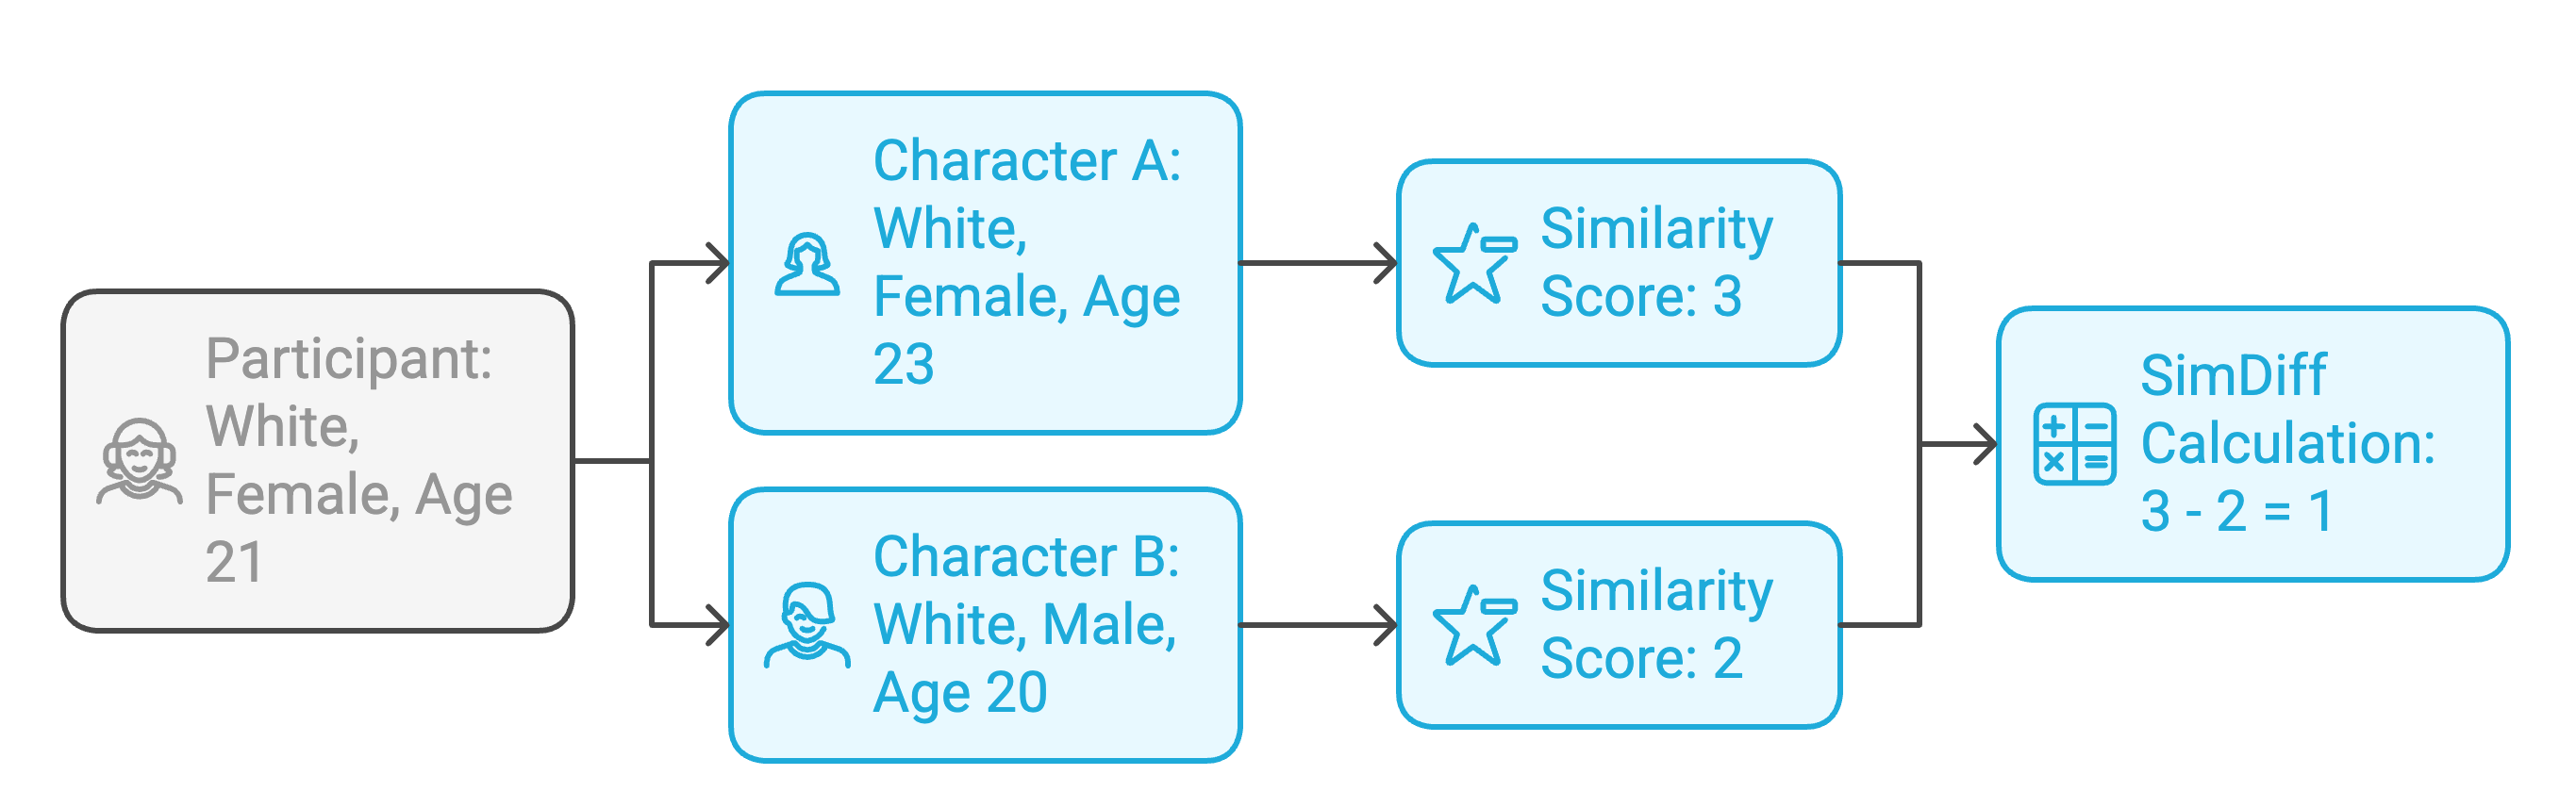
\includegraphics{figures/gap_example_new.png}

}

\end{figure}%

\subsection{Stimuli and Self-Similarity Gap
Manipulation}\label{stimuli-and-self-similarity-gap-manipulation}

Face images were licensed from the Chicago Face Database (CFD) and the
CFD-India subset. Only neutral-expression photos were used and resized
to a common resolution. Each image carried CFD metadata for age, gender,
and ethnicity as well as norming data for a range of face-based
features. Ma et al. (\citeproc{ref-ma2015chicago}{2015}) provides a
detailed description of the CFD and its norming procedures. Ethnicity
labels were restricted to five groups with ample coverage --
Black/African American, East Asian, Latino/Hispanic, South Asian, and
White -- to maintain balanced stimulus pools. Age was binned into four
brackets (18-24, 25-31, 32-38, 39-45) to equalize face counts across
brackets.

For every participant an eight-image pool was constructed so that
exactly two faces shared 0, 1, 2, or 3 of the participant's demographic
traits (ethnicity, gender, age bracket). Within each eight-image pool
there are \(\binom{8}{2}=28\) unique face pairs, so each participant
completed 28 choice trials. The self-similarity gap
Figure~\ref{fig-gap}, defined as the absolute difference in the number
of participant-shared traits between the left and right faces, served as
the primary predictor in all analyses.

\subsection{Trial Interface}\label{trial-interface}

On each trial two candidate faces appeared side by side with demographic
labels (race/ethnicity, sex, age) underneath. Left-right placement was
randomized. Participants selected a face by clicking a ``Left'' or
``Right'' button located below the images, and a one-line reminder of
the task goal appeared beneath the buttons. Choice and response time
were recorded from stimulus onset to button click.

\subsection{Participants}\label{participants}

One hundred individuals aged 18-45 were recruited on Prolific. The
sample was quota-balanced so that each of five ethnic categories
(Black/African American, East Asian, Latino/Hispanic, South Asian,
White) comprised 20 percent of participants and each gender comprised 50
percent. Participants were paid \$0.50 for a 3-5-minute session
(approximately \$10/hour). All participants completed the study and were
retained for analysis.

\subsection{Procedure}\label{procedure}

Participants first reported their own demographics and rated
self-perceived competitiveness on a 0-10 slider (not analyzed). The
eight-image pool was generated immediately after this survey. All
procedures were approved by the university IRB, and participants were
debriefed and compensated in full.

Participants were randomly assigned to one of two task framing
conditions. The low-stakes/affiliative frame described a relaxed
community project and instructed participants to choose teammates who
would make collaboration enjoyable and productive. The
high-stakes/performance frame described a grant competition and
instructed participants to choose teammates who would maximize the
team's chance of winning. For immersion, participants were told they had
been selected as team leader and could state their teammate preferences.
Before the first trial a three-second loading screen displayed a
progress bar and the message ``One moment. We are sorting you into a
lobby.'' Full wording for both instruction sets is provided in the
Supplementary Materials.

Participants then completed the 28 choice trials as described above.
After the final trial they completed a deception check asking whether
they expected a real follow-up game. Responses were recorded but not
used as exclusion criteria.

\subsection{Results}\label{results}

\subsubsection{Data Preparation}\label{data-preparation}

Raw data contained one record per trial (100 participants × 28 trials =
2,800 rows). For modeling we expanded each trial into two mirrored rows:
one treating the left face as the focal candidate and one treating the
right face as focal. This duplication (total 5,600 analytic rows)
removes any bias from the arbitrary left/right assignment and lets us
express the mixed-effects models with a single binary outcome:
\(\text{Preference} = 1\) if the focal face was chosen, \(0\) otherwise.
Each record contained the task framing condition (0 = affiliative, 1 =
performance), a raw/signed self-similarity gap (ranging from -3 to +3),
a binary choice flag (1 = focal face chosen), and log-transformed
reaction time (after trimming \textless{} 150 ms and \textgreater{} 10
s). Face metadata (ethnicity, gender, CFD trait norms) and participant
demographics were merged for subsequent models and robustness checks.

\subsubsection{Descriptive Overview}\label{descriptive-overview}

\begin{figure}

\caption{\label{fig-overall}Preference rate as a function of the
similarity between compared characters and the participant, measured
across all participants and conditions. \textbf{Left}: Preference rate
for the more-similar teammate as self-similarity gap increased. Error
bars represent bootstrapped 95\% confidence intervals. Horizontal dashed
line indicates chance level (50\%). \textbf{Right}: Preference rates
across counts of shared features to each participant for compared
character. Color intensity indicates the probability of selecting the
more-similar character, with darker colors indicating higher
probabilities. Cells where focal character shares fewer features with
participant than the competitor are not shown.}

\begin{minipage}{0.50\linewidth}
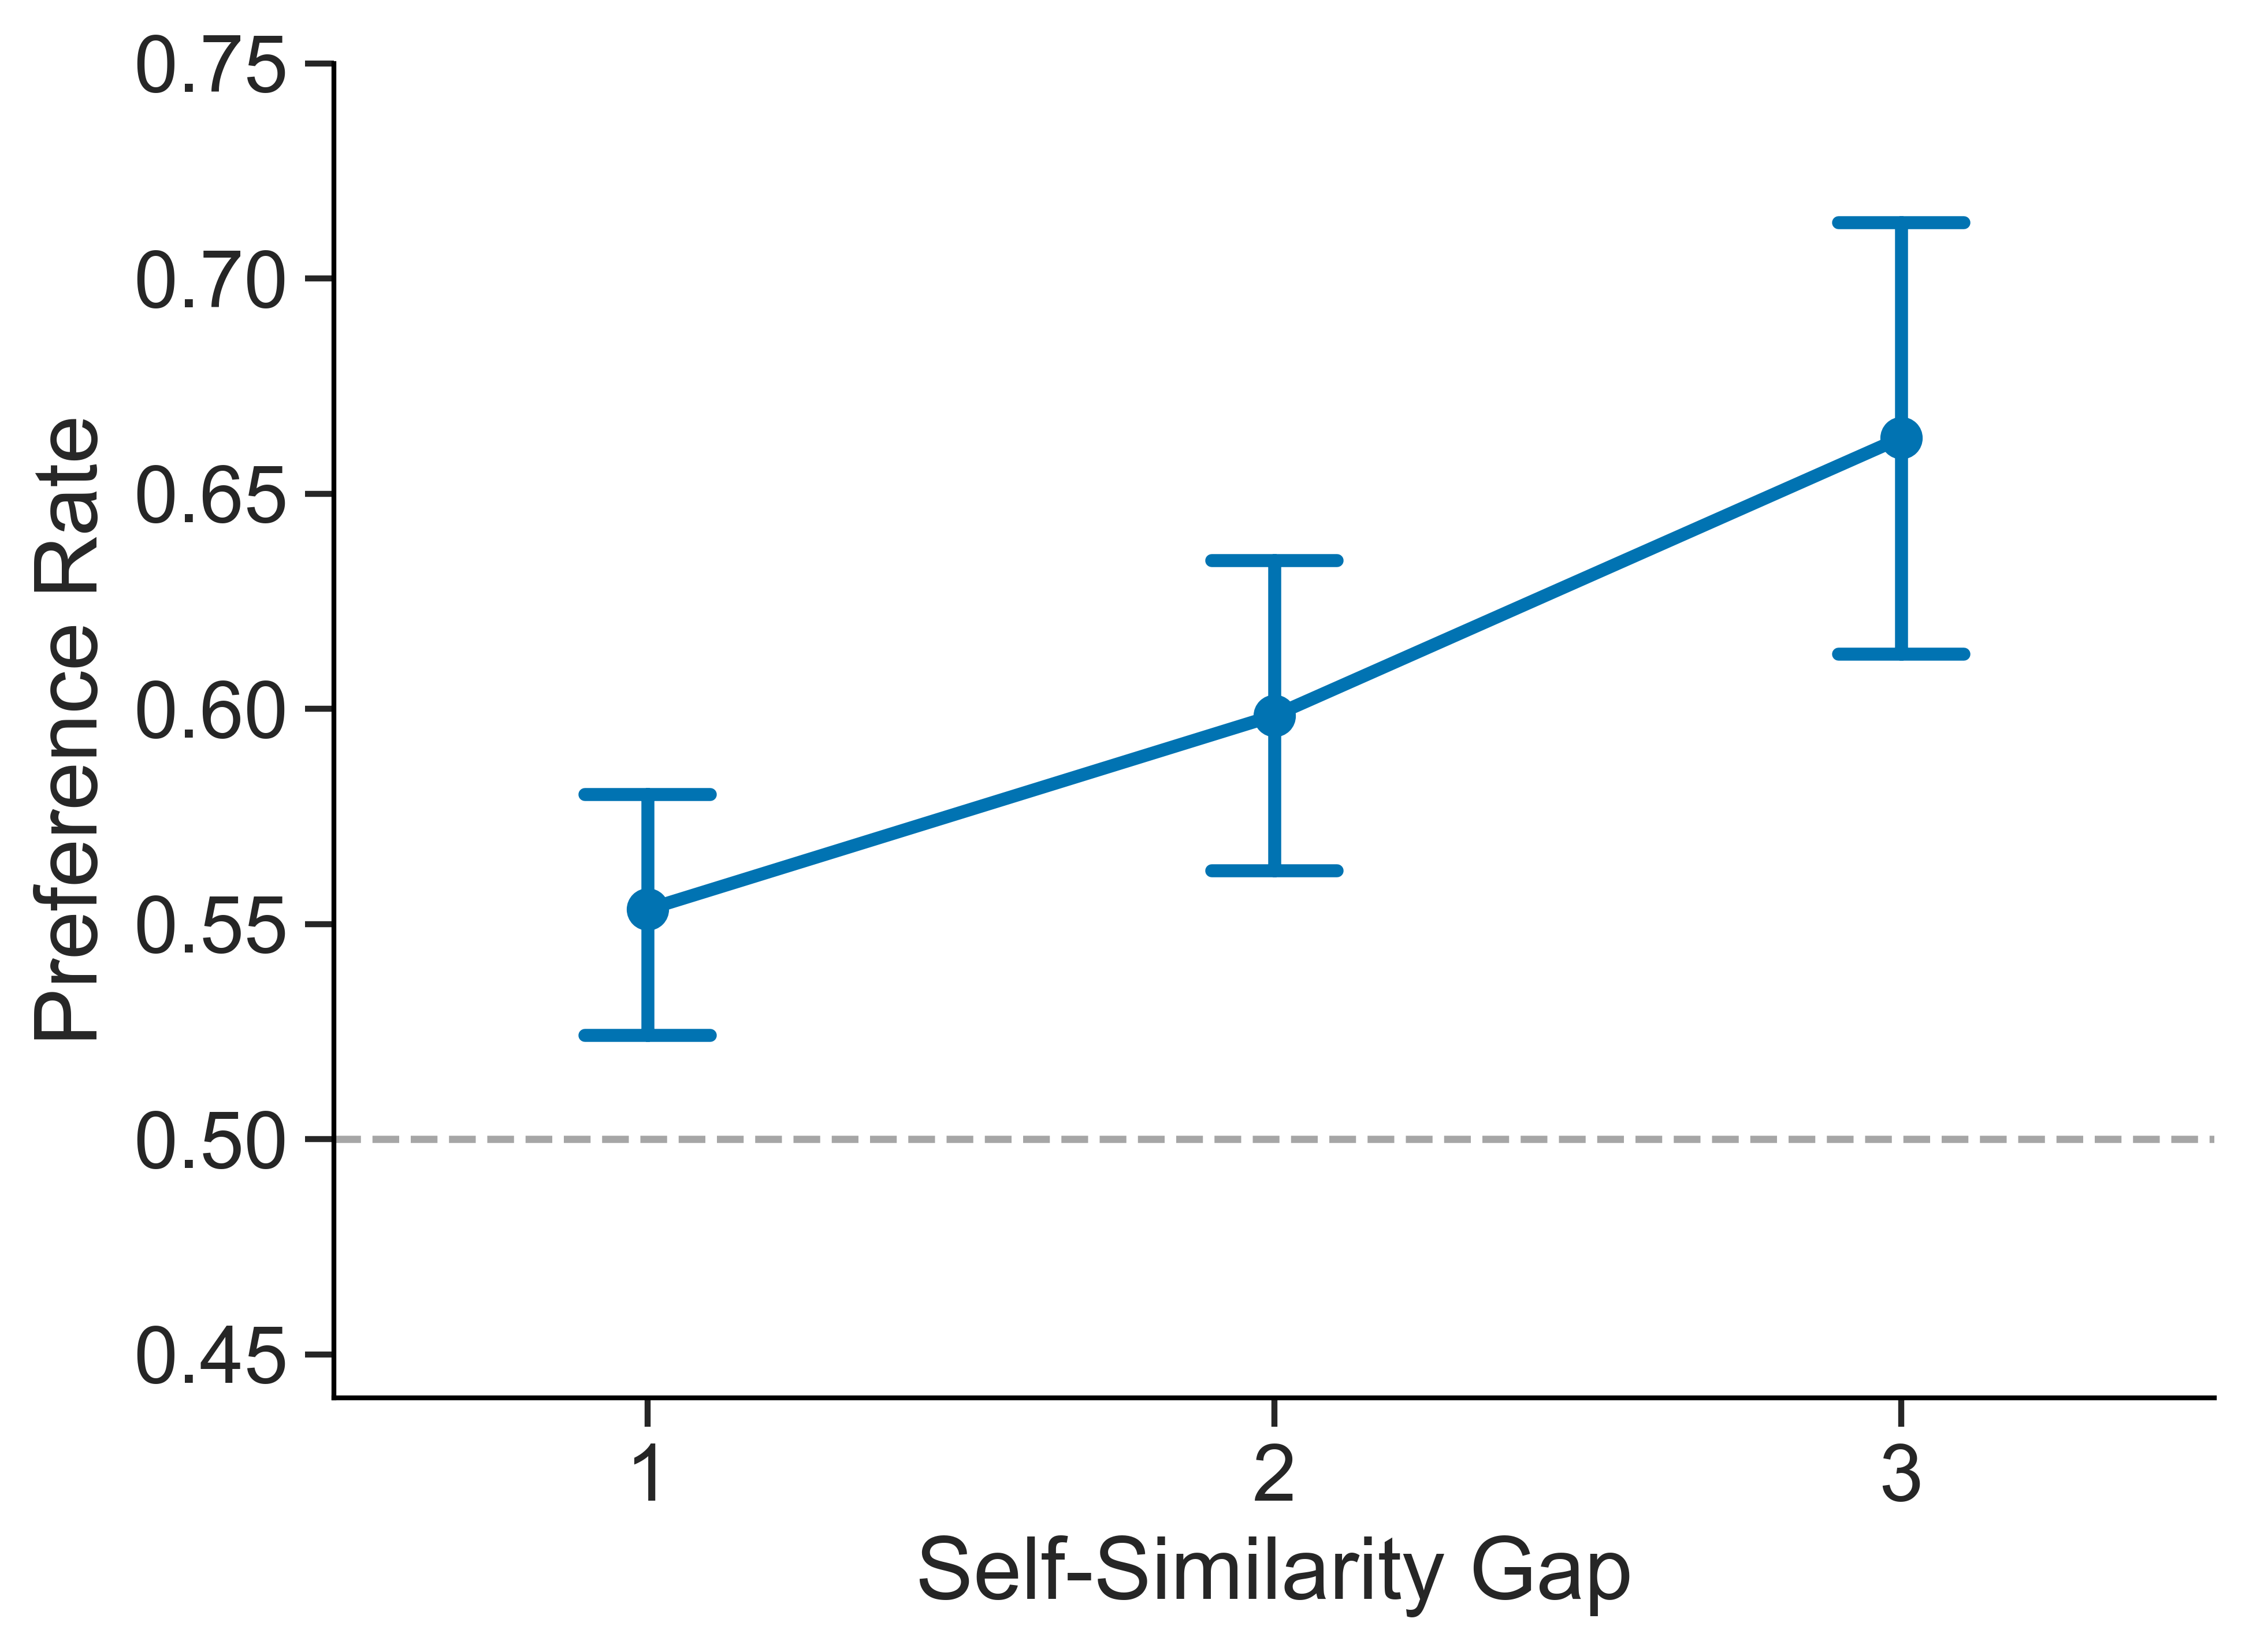
\includegraphics{figures/pointplot_chosen_vs_simDiff.png}\end{minipage}%
%
\begin{minipage}{0.50\linewidth}
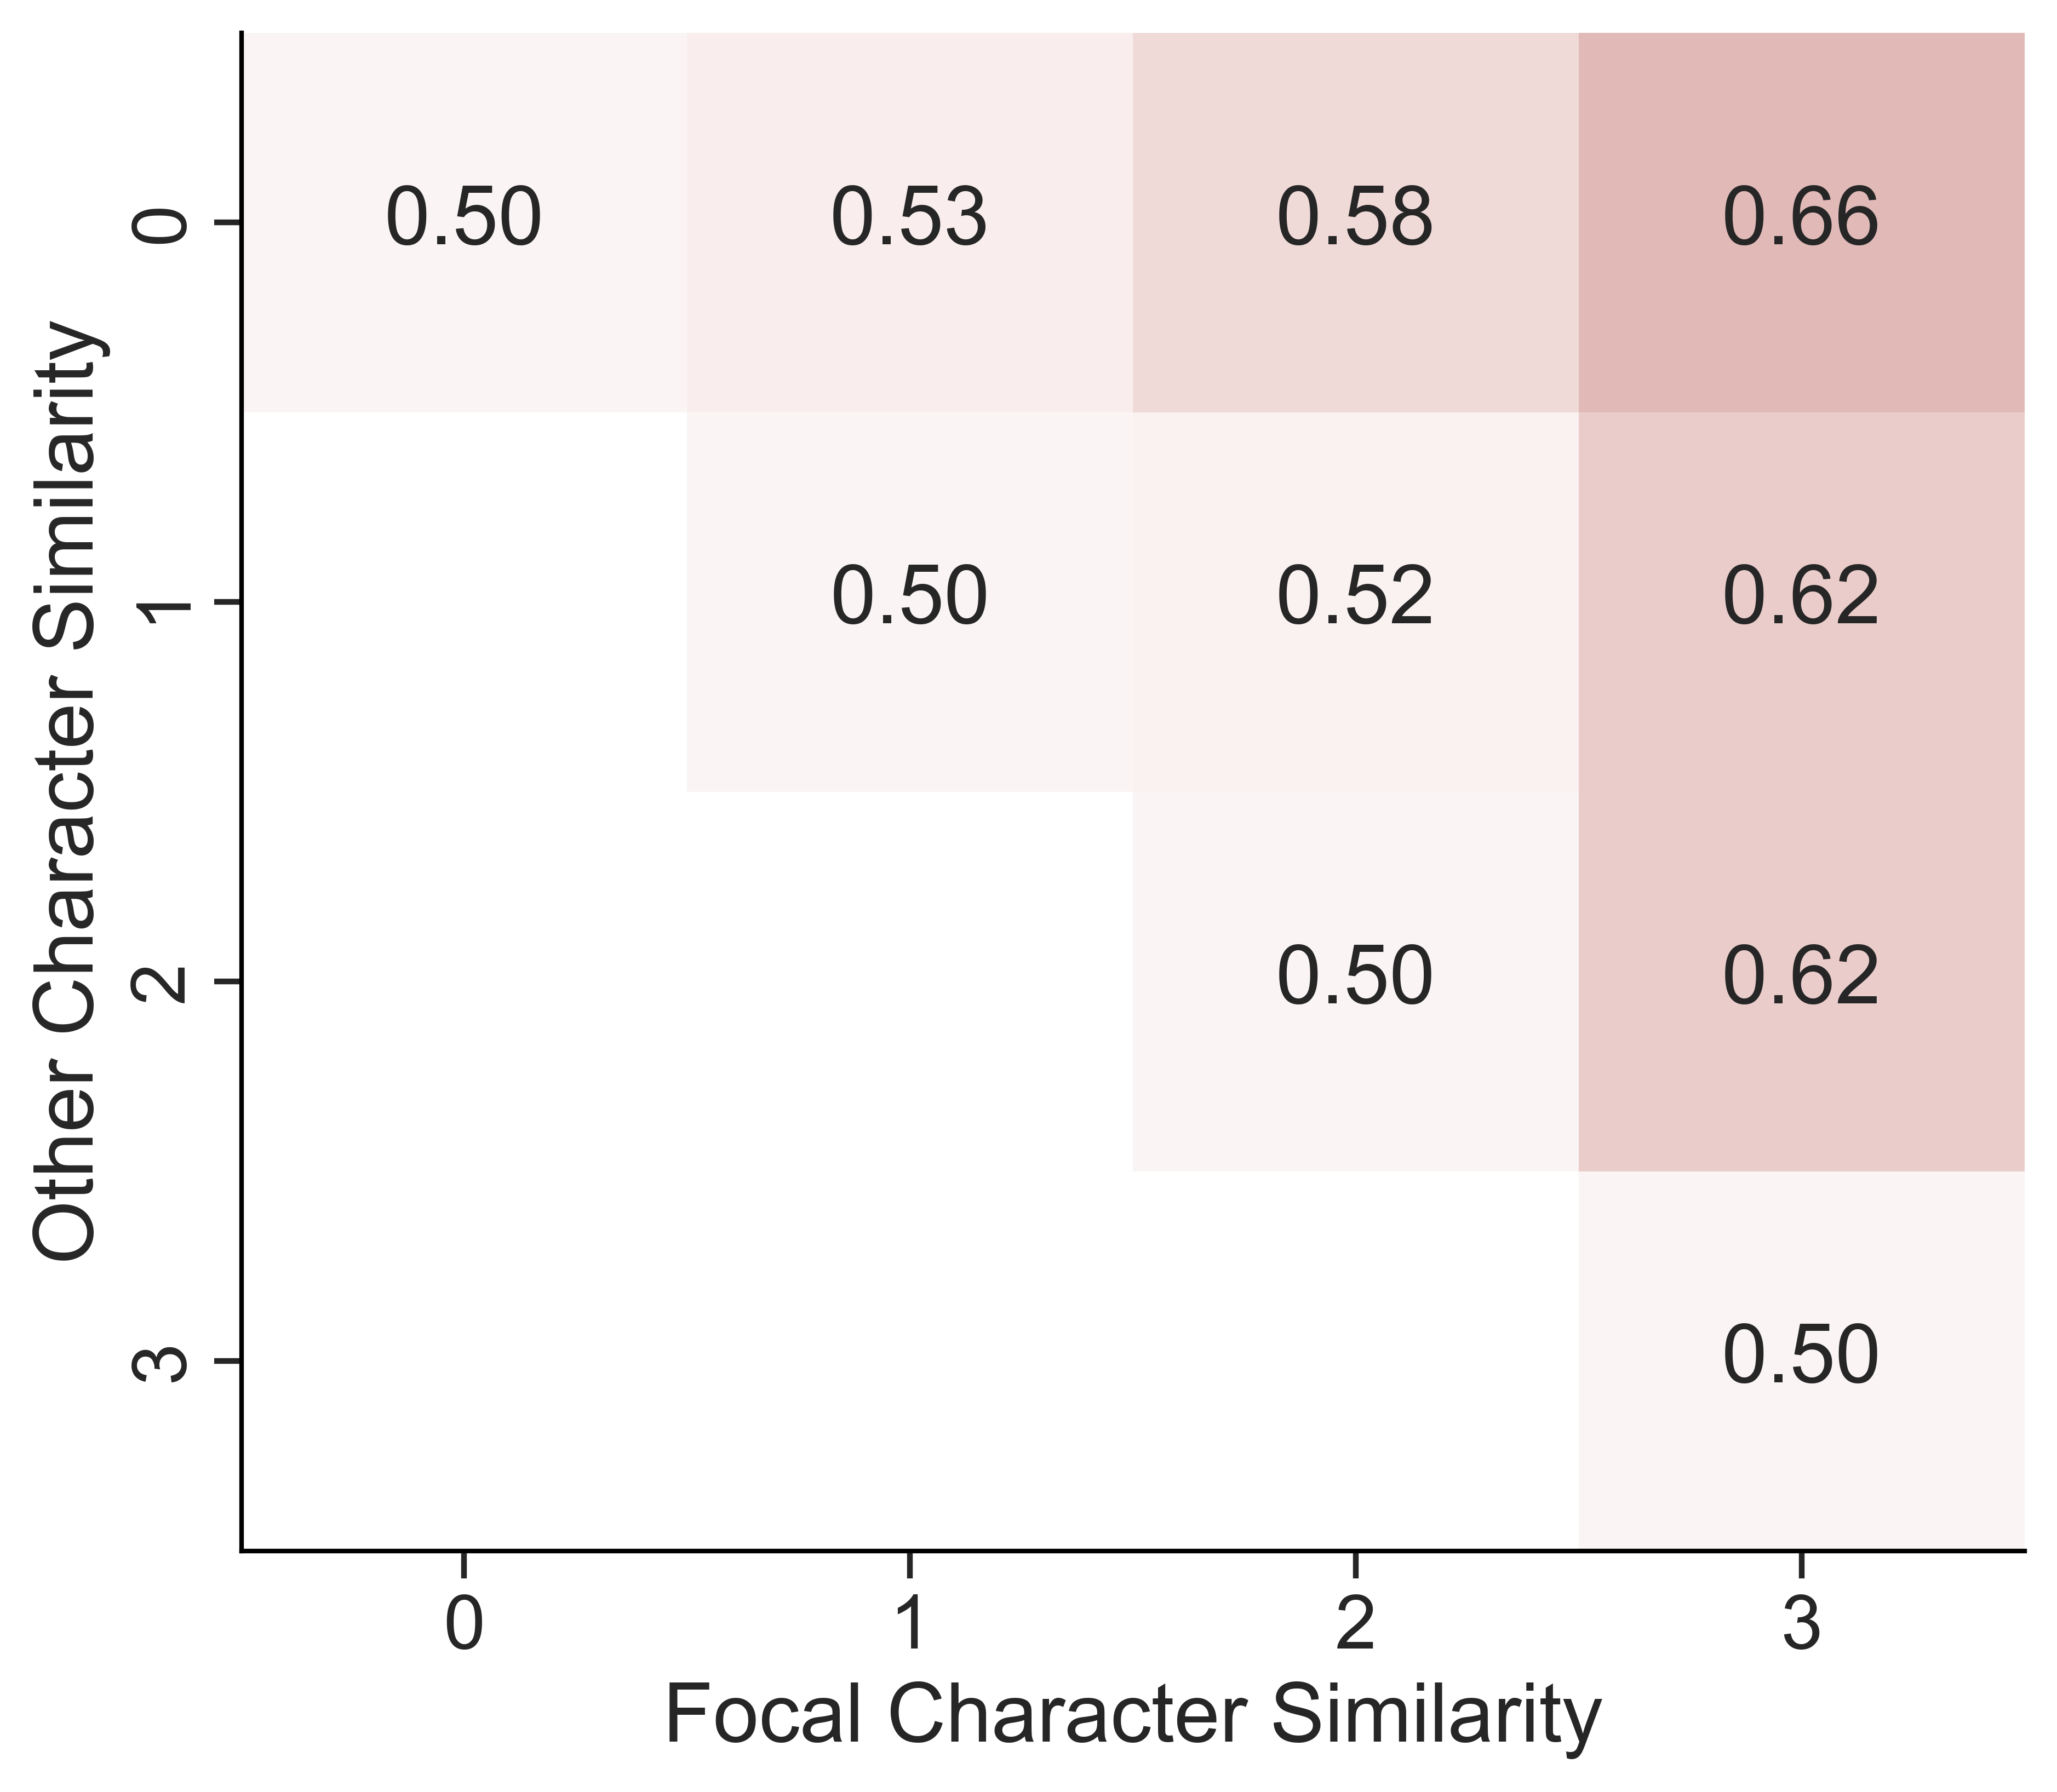
\includegraphics{figures/heatmap_preferences.png}\end{minipage}%

\end{figure}%

\begin{figure}

\caption{\label{fig-pointsplit}Point plots showing the preference rate
for the more-similar teammate across all participants as self-similarity
gap increased, split by framing condition (low-stakes/affiliative
vs.~high-stakes/performance). Error bars represent bootstrapped 95\%
confidence intervals. Horizontal dashed line indicates chance level
(50\%).}

\begin{minipage}{\linewidth}

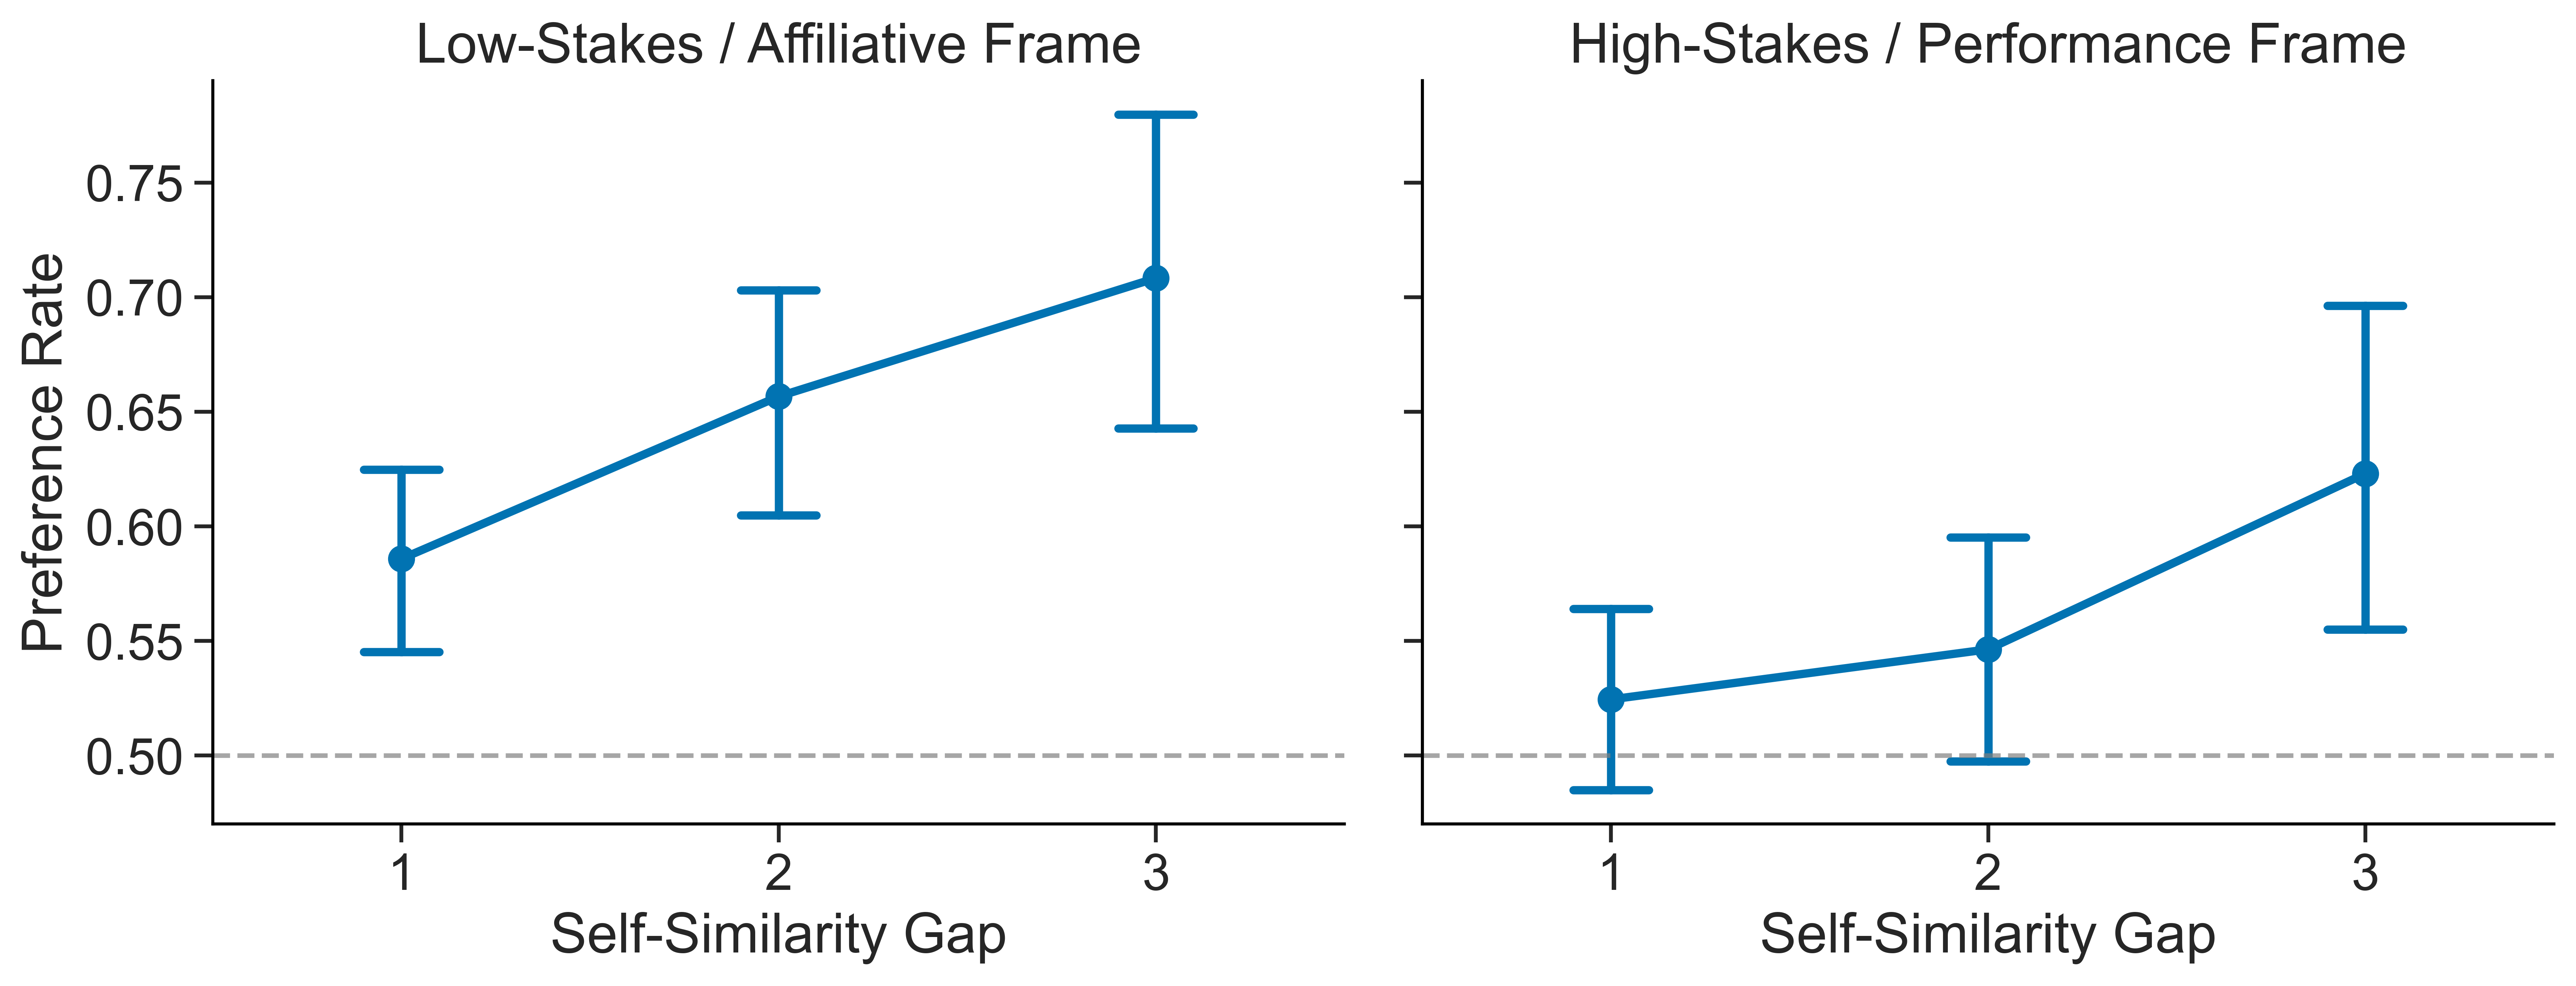
\includegraphics{figures/pointplot_chosen_vs_simDiff_condition.png}

\end{minipage}%

\end{figure}%

\begin{figure}

\caption{\label{fig-heatmapsplit}Preference rates across counts of
shared features to each participant for compared character, split by
framing condition (low-stakes/affiliative vs.~high-stakes/performance).
Color intensity indicates the probability of selecting the more-similar
character, with darker colors indicating higher probabilities. Cells
where focal character shares fewer features with participant than the
competitor are not shown.}

\begin{minipage}{\linewidth}

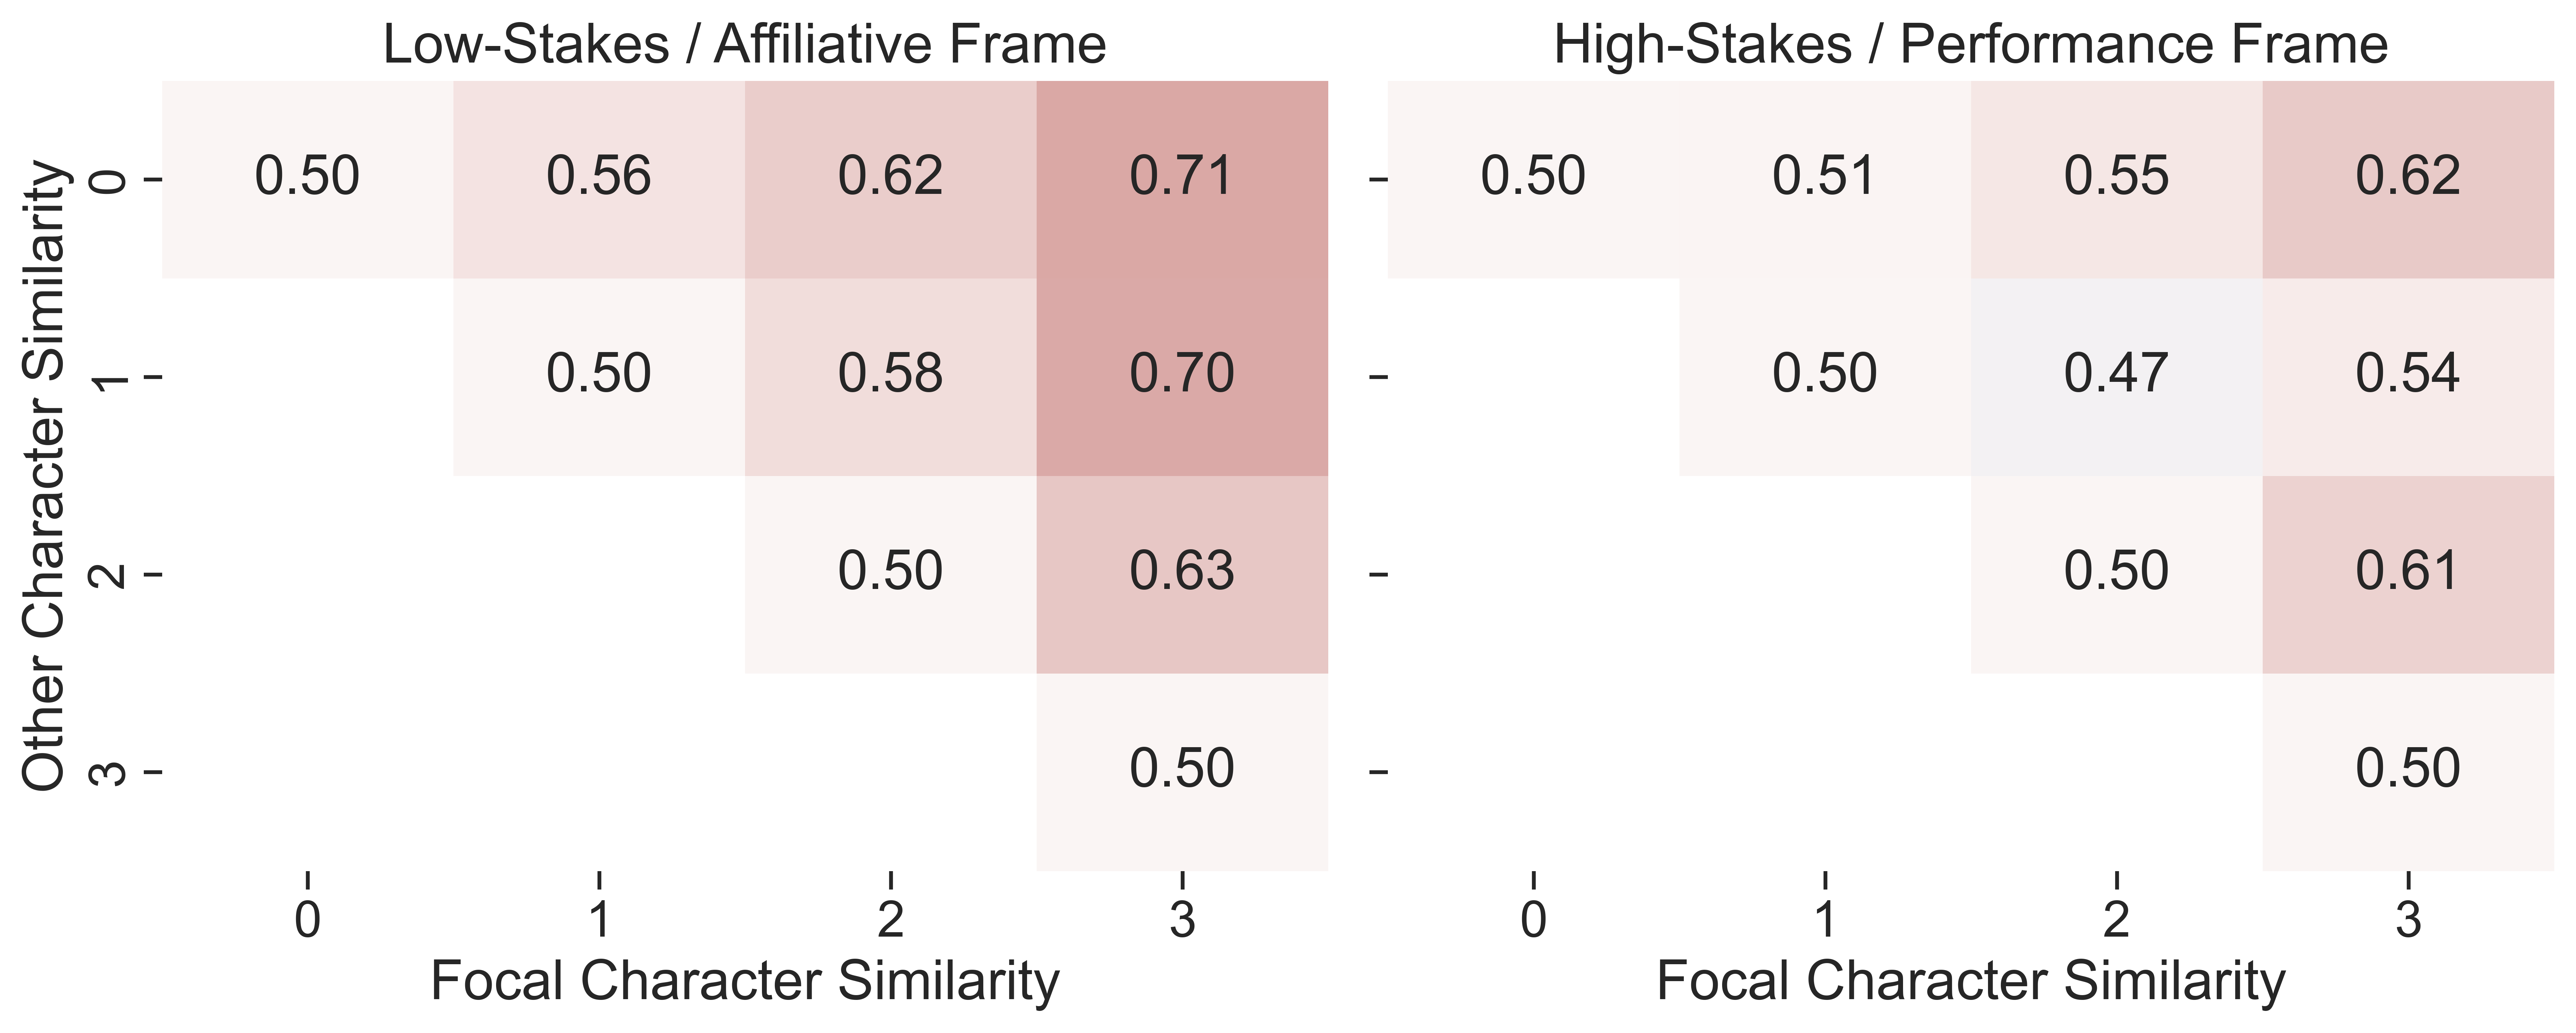
\includegraphics{figures/heatmaps_by_condition.png}

\end{minipage}%

\end{figure}%

\begin{figure}

\caption{\label{fig-rtpointsplit}Point plots showing the mean log
reaction time for the more-similar teammate across all participants as
self-similarity gap increased, split by framing condition
(low-stakes/affiliative vs.~high-stakes/performance). Error bars
represent bootstrapped 95\% confidence intervals. Horizontal dashed line
indicates chance level (50\%).}

\begin{minipage}{\linewidth}

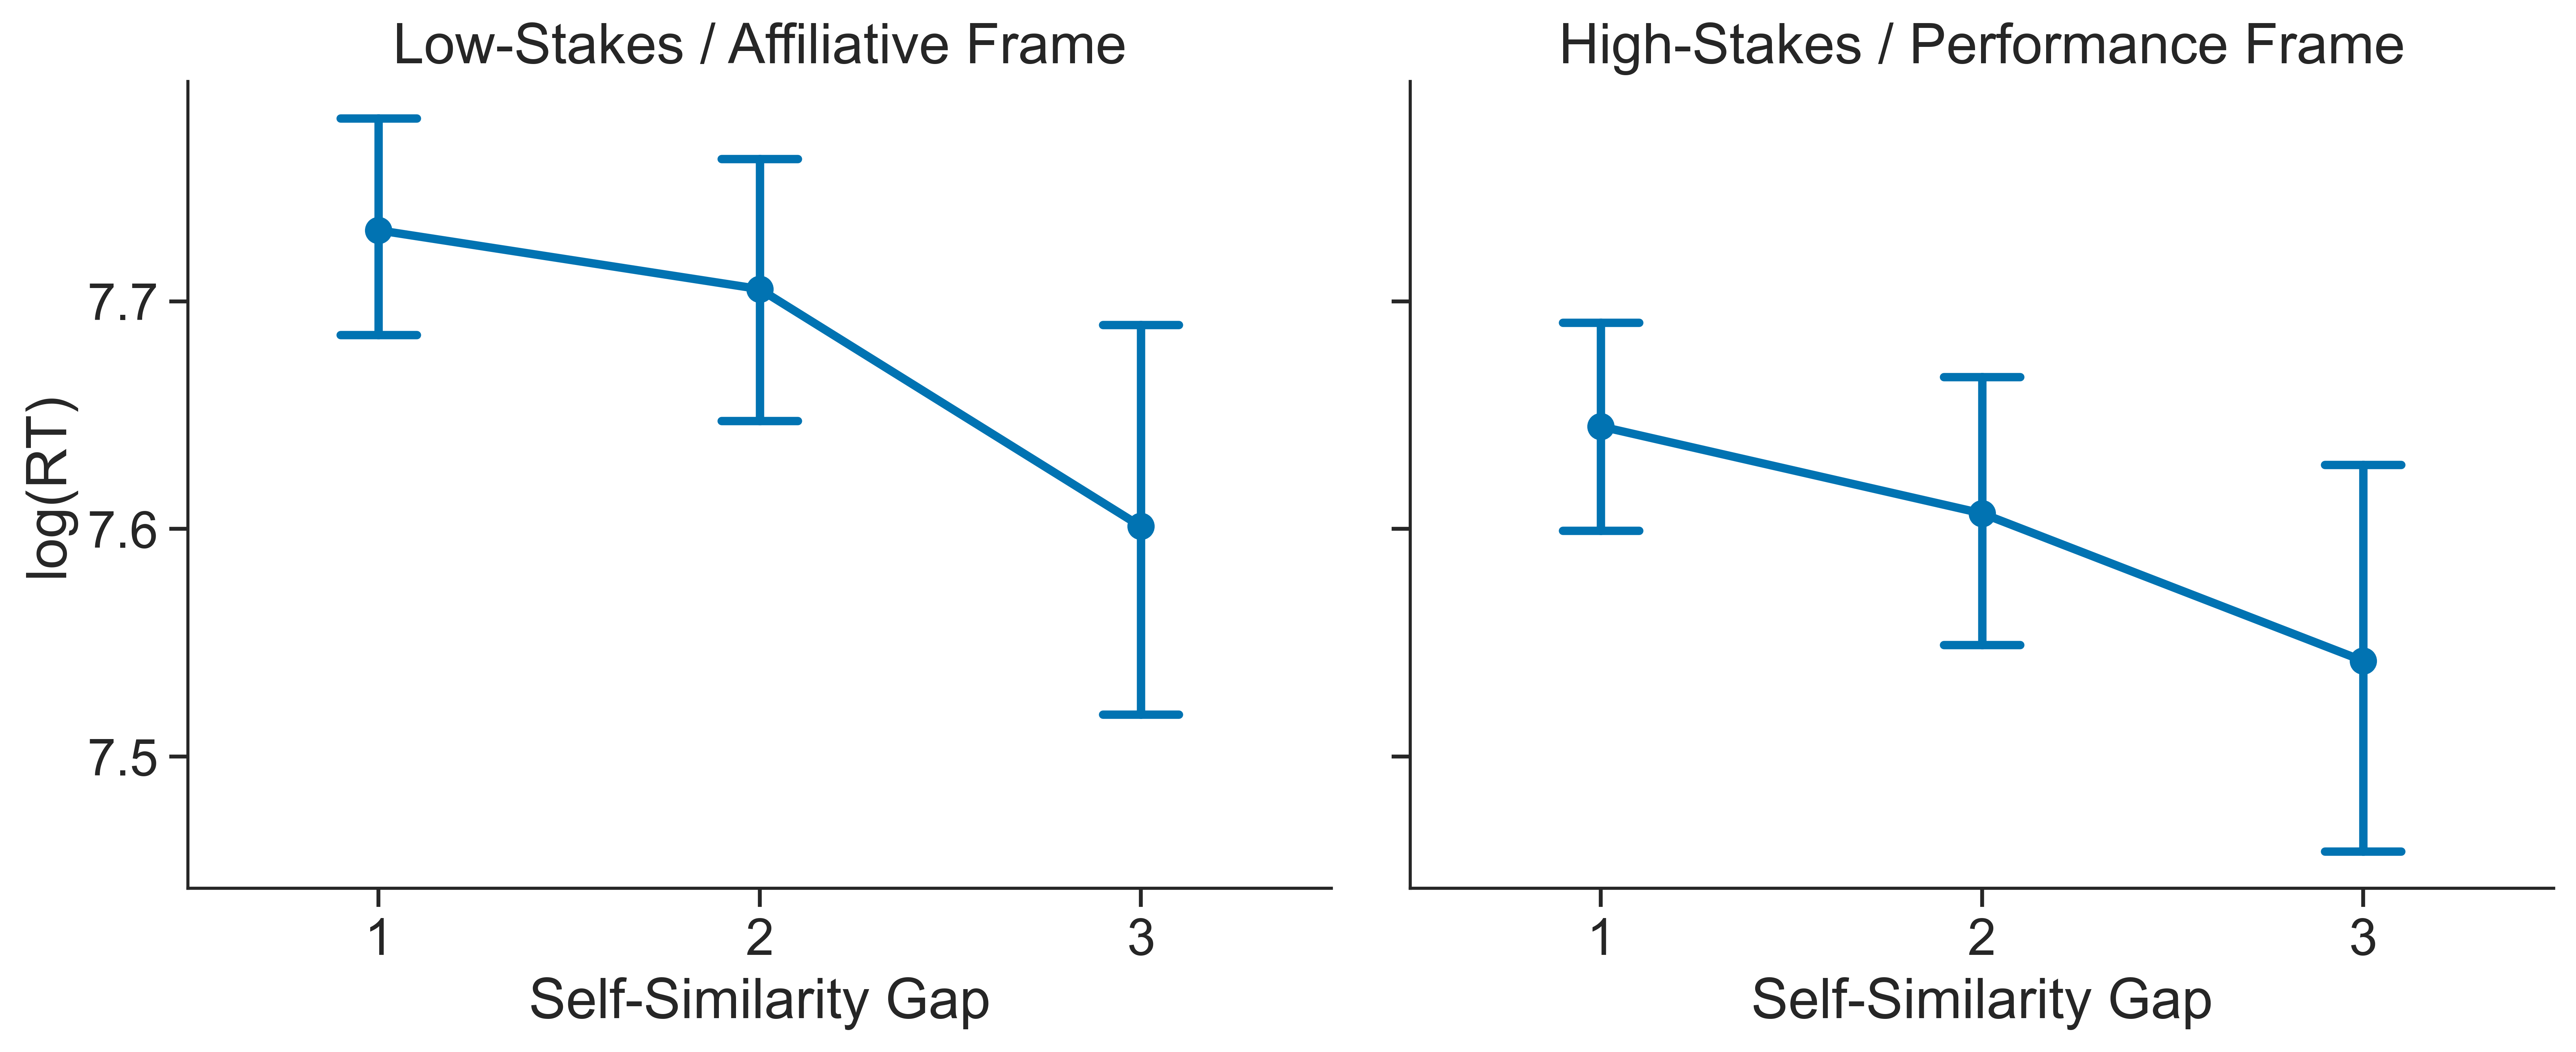
\includegraphics{figures/pointplot_logRT_vs_simDiff_byCondition.png}

\end{minipage}%

\end{figure}%

First, we seek to characterize the overall effect of demographic
self-similarity on team formation. Participants' tendency to choose
more-similar teammates is visualized using both point plots and
heatmaps. Point plots show the probability of selecting the focal
character as a function of self-similarity gap, which is the absolute
difference in the number of demographic features shared with the
participant between the focal character and the competitor. For
visualization purposes, the focal character is always the more-similar
of the two, restricting self-similarity gap values to the non-negative
range (0, 1, 2, 3). Heatmaps represent preference probabilities for each
possible combination of the number of features the participant shares
with the focal character and with the competitor, yielding a 4×4 grid of
probabilities where the top-right cell corresponds to the maximum
self-similarity gap of 3.

Figure~\ref{fig-overall} summarises the aggregate pattern. The point
plot (left) shows a monotonic rise in the probability of selecting the
more-similar candidate as the self-similarity gap increases from 0 to 3,
with 95\% bootstrap CIs well above chance at every level and a peak
preference of 0.66 at the maximum gap. The accompanying heat-map (right)
confirms that this gradient holds across the full 4 × 4 matrix of
similarity counts.

When the data are split by framing condition
(Figure~\ref{fig-pointsplit} and Figure~\ref{fig-heatmapsplit}), the
homophily gradient is visibly steeper under the low-stakes / affiliative
frame than under the high-stakes / performance frame. In the affiliative
condition, preference for the more-similar face is above chance at every
gap and rises steadily with each additional shared trait. In the
performance condition the increase is muted and less consistent,
suggesting that participants down-weight self-similarity when
performance incentives are foregrounded.

Figure~\ref{fig-rtpointsplit} shows that decision speed mirrors the
preference data: selections become faster as the self-similarity gap
widens, but chiefly in the affiliative frame. When the task emphasises
performance, reaction times less consistently decrease with increasing
self-similarity gap, suggesting that self-similarity is less decisive in
the high-stakes context.

\subsubsection{Mixed Effects Logistic
Regression}\label{mixed-effects-logistic-regression}

\begin{table}

{\caption{{Mixed-effects logistic model predicting choice of the
more-similar teammate. Odds ratios \textgreater{} 1 indicate higher odds
of choosing the focal face.}{\label{tbl-pref}}}
\vspace{-20pt}}

\begin{longtable}[]{@{}
  >{\raggedright\arraybackslash}p{(\columnwidth - 10\tabcolsep) * \real{0.3056}}
  >{\raggedleft\arraybackslash}p{(\columnwidth - 10\tabcolsep) * \real{0.1389}}
  >{\raggedleft\arraybackslash}p{(\columnwidth - 10\tabcolsep) * \real{0.1389}}
  >{\raggedleft\arraybackslash}p{(\columnwidth - 10\tabcolsep) * \real{0.1389}}
  >{\raggedleft\arraybackslash}p{(\columnwidth - 10\tabcolsep) * \real{0.1389}}
  >{\raggedleft\arraybackslash}p{(\columnwidth - 10\tabcolsep) * \real{0.1389}}@{}}
\toprule\noalign{}
\begin{minipage}[b]{\linewidth}\raggedright
Fixed Effect
\end{minipage} & \begin{minipage}[b]{\linewidth}\raggedleft
Estimate (\(\beta\))
\end{minipage} & \begin{minipage}[b]{\linewidth}\raggedleft
SE
\end{minipage} & \begin{minipage}[b]{\linewidth}\raggedleft
z
\end{minipage} & \begin{minipage}[b]{\linewidth}\raggedleft
p
\end{minipage} & \begin{minipage}[b]{\linewidth}\raggedleft
Odds Ratio exp(\(\beta\))
\end{minipage} \\
\midrule\noalign{}
\endhead
\bottomrule\noalign{}
\endlastfoot
(Intercept) & 0.010 & 0.0639 & 0.163 & 0.871 & 1.01 \\
Self-Similarity Gap & 0.358 & 0.0735 & 4.87 & \(1.1 \times 10^{-6}\) &
1.43 \\
High-Stakes (vs.~Low-Stakes) & --0.025 & 0.0723 & --0.350 & 0.727 &
0.98 \\
Gap × Frame (Interaction) & --0.140 & 0.0591 & --2.37 & \textbf{0.018} &
0.87 \\
\end{longtable}

\end{table}

\begin{table}

{\caption{{Mixed-effects linear model predicting log-transformed
reaction time.}{\label{tbl-rt-fixed}}}
\vspace{-20pt}}

\begin{longtable}[]{@{}
  >{\raggedright\arraybackslash}p{(\columnwidth - 8\tabcolsep) * \real{0.2568}}
  >{\raggedleft\arraybackslash}p{(\columnwidth - 8\tabcolsep) * \real{0.2162}}
  >{\raggedleft\arraybackslash}p{(\columnwidth - 8\tabcolsep) * \real{0.1757}}
  >{\raggedleft\arraybackslash}p{(\columnwidth - 8\tabcolsep) * \real{0.1757}}
  >{\raggedleft\arraybackslash}p{(\columnwidth - 8\tabcolsep) * \real{0.1757}}@{}}
\toprule\noalign{}
\begin{minipage}[b]{\linewidth}\raggedright
Fixed Effect
\end{minipage} & \begin{minipage}[b]{\linewidth}\raggedleft
Estimate (\(\beta\))
\end{minipage} & \begin{minipage}[b]{\linewidth}\raggedleft
SE
\end{minipage} & \begin{minipage}[b]{\linewidth}\raggedleft
\(t\)
\end{minipage} & \begin{minipage}[b]{\linewidth}\raggedleft
\(p\)
\end{minipage} \\
\midrule\noalign{}
\endhead
\bottomrule\noalign{}
\endlastfoot
(Intercept) & 7.780 & 0.0429 & 181.26 & \(< 2 \times 10^{-16}\) \\
Self-Similarity Gap & \(-0.040\) & 0.0118 & \(-3.43\) &
\textbf{0.00061} \\
\end{longtable}

\end{table}

To more completely test whether demographic self-similarity predicts
teammate preference and whether this effect is modulated by contextual
framing, we fit a generalized linear mixed-effects model (logistic) with
self-similarity gap, framing condition (casual vs.~competitive), and
their interaction as fixed effects. In line with prior definitions,
self-similarity gap was calculated as the number of demographic features
(race, sex, and age) that the chosen character shared with the
participant relative to the unchosen alternative. Here, the
self-similarity gap was allowed to take on negative values when the
unchosen character shared more features with the participant than the
chosen character. By contrast, a higher self-similarity gap indicates
that the selected character was more demographically similar to the
participant. The model included a random intercept for character to
capture baseline differences in character popularity independent of
demographic attributes. Importantly, we also introduced a random slope
for self-similarity gap at the participant level, allowing the strength
of homophily to vary by individual. The model formula was:

\phantomsection\label{eq-mixed-effects}
\[
\text{Preference} \sim \text{Self-Similarity Gap} \times \text{Framing Condition}
\] \[
+ (1 \mid \text{Character}) +\bigl(0 + \text{Self-Similarity Gap} \mid \text{Participant}\bigr)
\]

Specifying a participant-level slope for the self-similarity gap term
yielded a substantially improved fit over a model without the term (AIC
= 7210.4, BIC = 7243.5 → AIC = 6933.9, BIC = 6973.6), and the final
model described meaningful variance in both random effects. The model
confirmed that participants were significantly more likely to choose
characters who were demographically similar to themselves (\(\beta\) =
0.358, p == \(1.1 \times 10^{6}\)). A significant interaction effect
between self-similarity gap and framing condition was also found
(\(\beta\) = -0.14, z=-2.37, p = 0.018), suggesting that participants
were less influenced by self-similarity under a high-stakes/performance
framing compared to a low-stakes/affiliative framing.

The random slope variance for self-similarity gap was substantial (Var =
0.193, SD = 0.439), indicating that participants differed in how
strongly they weighted demographic self-similarity when selecting
teammates. Some exhibited strong homophily, while others showed weaker
or even reversed preferences. The random intercept variance for
character also remained large (Var = 0.636, SD = 0.798), suggesting
persistent character-level biases unrelated to self-similarity.

As a follow-up analysis, we decomposed the summed gap into separate
race-, age-, and gender-match differences and fit an otherwise analogous
logistic mixed model with participant-level slopes for each component
(see Table~\ref{tbl-multisimdiff-components}). Race- and age-match
differences both positively predicted selection of the focal candidate
(\(\beta\)s = 0.89 and 0.60, ps \textless{} .05), whereas the
gender-match term was smaller and less precise (\(\beta\) = 0.46, p =
.12). This suggests that the aggregate self-similarity effect was not
reducible to race matching alone, although the clearest contributions
came from race and age rather than gender.

We analysed decision speed with a linear mixed model in which
log-transformed RT (milliseconds) was regressed on the signed
self-similarity gap, with a random intercept for each participant.
Character-level random effects were not included due to low variance in
the character intercepts.

\[
log(\mathrm{RT}) \sim \text{Self-Similarty Gap} + ( 1\mid\text{Participant})
\]

As Table~\ref{tbl-rt-fixed} shows, the gap coefficient was negative
(\(\beta\) = --0.040 ± 0.012 SE, t = --3.43, p = .00061).
Back-transforming the estimate, each one-unit increase in gap multiplied
RT by exp(--0.040) \(\approx\) 0.96 -- about a 4\% reduction in decision
time per additional shared trait difference. Given a baseline of
\textasciitilde2.4 s (exp \(\beta_0 \approx 2 396\) ms), this translates
to roughly 90--100 ms faster responses for gap = 2 versus gap = 1, and
\textasciitilde180 ms for gap = 3 versus gap = 1. Thus, the same
homophily cue that boosts choice probability also quickens decisions,
consistent with the idea that larger self-similarity gaps make the
choice easier to resolve. Participant intercepts further showed
appreciable heterogeneity (Var = 0.145, SD = 0.381), indicating baseline
speed differences across individuals.

\subsubsection{Preferences Independent of
Self-Similarity}\label{preferences-independent-of-self-similarity}

In our mixed-effects modeling of teammate preference, we observed a
substantial amount of variability in the random intercept for character,
indicating that some characters were consistently preferred or avoided
by participants, independent of their demographic self-similarity. We
examined this baseline preference for characters through two
perspectives. First, we assessed whether participants exhibited general
preferences for specific demographic groups, independent of
self-similarity, such as specific age groups or ethnicities. This could
explain character-level biases in terms of general attraction or
aversion to certain groups, rather than a specific preference for
self-similarity. Second, we applied CFD trait-norms to assess whether
participants preferred characters that tended elicit specific trait
impressions, such as competence or threat. This could indicate that
participants were selecting characters based on perceived attributes
rather than or as part of a broader tendency toward homophily.

\subsubsection{Demographic Preferences}\label{demographic-preferences}

To assess demographic preferences independent of self-similarity, we fit
a demographic-only mixed-effects model in which choice was predicted by
the candidate's race, age, and gender, each crossed with framing
condition and controlling for a random intercept for character:

\[ 
\text{Preference} \sim 
\bigl(\text{Race} + \text{Age} + \text{Gender}\bigr) \times \text{Frame} + (1 \mid \text{Character})
\]

where the reference category is a Black, female face at the sample-mean
age, shown in the affiliative frame. Character ID remained as a random
intercept (Var = 0.56, SD = 0.75). The fixed-effects estimates are
summarised in Table~\ref{tbl-demo-fixed}.

\begin{table}

{\caption{{Fixed effects from the demographic-only model predicting
choice of the focal face.}{\label{tbl-demo-fixed}}}
\vspace{-20pt}}

\begin{longtable}[]{@{}
  >{\raggedright\arraybackslash}p{(\columnwidth - 8\tabcolsep) * \real{0.2000}}
  >{\raggedleft\arraybackslash}p{(\columnwidth - 8\tabcolsep) * \real{0.2000}}
  >{\raggedleft\arraybackslash}p{(\columnwidth - 8\tabcolsep) * \real{0.2000}}
  >{\raggedleft\arraybackslash}p{(\columnwidth - 8\tabcolsep) * \real{0.2000}}
  >{\raggedleft\arraybackslash}p{(\columnwidth - 8\tabcolsep) * \real{0.2000}}@{}}
\toprule\noalign{}
\begin{minipage}[b]{\linewidth}\raggedright
Fixed Effect
\end{minipage} & \begin{minipage}[b]{\linewidth}\raggedleft
Estimate (\(\beta\))
\end{minipage} & \begin{minipage}[b]{\linewidth}\raggedleft
SE
\end{minipage} & \begin{minipage}[b]{\linewidth}\raggedleft
\(z\)
\end{minipage} & \begin{minipage}[b]{\linewidth}\raggedleft
\(p\)
\end{minipage} \\
\midrule\noalign{}
\endhead
\bottomrule\noalign{}
\endlastfoot
(Intercept) & 1.413 & 0.281 & 5.02 & \(5.2\times10^{-7}\) \\
East-Asian & 0.211 & 0.183 & 1.15 & .25 \\
Latino & --0.300 & 0.202 & --1.49 & .14 \\
South-Asian & --0.394 & 0.194 & --2.03 & \textbf{.042} \\
White & --0.356 & 0.176 & --1.99 & \textbf{.047} \\
High-Stakes / Performance frame & --0.471 & 0.318 & --1.48 & .14 \\
Age (per year) & --0.0349 & 0.0074 & --4.74 & \(2.2\times10^{-6}\) \\
Male (vs.~female) & --0.295 & 0.121 & --2.43 & \textbf{.015} \\
South-Asian × High-Stakes & 0.489 & 0.233 & 2.10 & \textbf{.036} \\
all other Race×Frame and trait×Frame interactions & --- & --- & &
\(>.12\) \\
\end{longtable}

\end{table}

South-Asian and White faces were selected less often than Black faces
(odds ratios \(\approx\) 0.67 and 0.70, respectively; ps \textless{}
.05), whereas East-Asian and Latino faces did not differ reliably from
the reference category. Each additional year of target age lowered the
odds of selection by about 3\% (\(\beta\) = --0.035, p \textless{}
.001), indicating a general preference for younger teammates. Finally,
male faces were chosen less frequently than female faces (\(\beta\) =
--0.30, p = .015).

Framing the task as high-stakes had no impact on these baseline race,
age, or gender effects, apart from a modest attenuation of the
South-Asian disadvantage (interaction \(\beta\) = 0.49, p = .036).
Because these demographic biases remain essentially stable across
frames, the Gap × Frame interaction observed in the homophily model must
reflect a genuine shift in the weighting of self-similarity, not a
wholesale change in attraction or aversion to particular groups. A
supplementary extension adding candidate-race × participant-race
interactions indicated that these apparent race disadvantages were not
shared uniformly across participant groups. The South-Asian-face
disadvantage was concentrated among Black participants, whereas the
White-face disadvantage appeared mainly among Black and South-Asian
participants (see Table~\ref{tbl-demo-participant-race}; excluding one
Multiracial and one Other participant).

\subsubsection{Trait Norms}\label{trait-norms}

The main framing manipulation varied both goal type and stakes
simultaneously: the affiliative condition was also low-stakes, whereas
the performance condition was also high-stakes. As a result, the Gap ×
Frame interaction alone is open to multiple interpretations. It could
reflect a general increase in caution under high stakes, a more specific
shift in which cues are used to evaluate potential teammates, or both.
To narrow that ambiguity, we analyzed trait norms from the Chicago Face
Database (CFD) to test whether the two frames altered how facial cues
were weighted during teammate selection. Each face in the CFD has been
rated by norming samples on a range of traits, including attractiveness,
dominance, happiness, sadness, threat, and trustworthiness.

For each trial, we computed a signed focal-minus-opponent difference
score for each trait. Positive values indicate that the focal face was
rated higher than the comparison face on that trait, whereas negative
values indicate that the focal face was rated lower. We then fit six
separate logistic mixed models, one per trait, predicting whether the
focal face was chosen from trait difference, framing condition, and
their interaction, with a random intercept for character:

\[
\text{Preference} \sim \text{Trait Difference} \times \text{Frame} + (1 \mid \text{Character})
\]

The full set of fixed-effect estimates is reported in
Table~\ref{tbl-trait-norms}. Across the six models, the clearest
condition-sensitive effect concerned threat. More threatening focal
faces were substantially less likely to be chosen in the affiliative
frame (\(\beta\) = -0.435, SE = 0.054, z = -8.00, p \textless{} .001),
and this avoidance was significantly attenuated in the
high-stakes/performance frame (Threat × Frame: \(\beta\) = 0.184, SE =
0.071, z = 2.59, p = .010, BH-adjusted p = .029). Facial sadness showed
a similar interaction (\(\beta\) = 0.174, SE = 0.064, z = 2.72, p =
.007, BH-adjusted p = .029). By contrast, the smaller attractiveness
interaction did not remain significant after correction for the six
trait-by-frame tests (raw p = .029, BH-adjusted p = .059).

\subsection{Discussion}\label{discussion}

Experiment 1 shows that demographic self-similarity influenced teammate
selection most strongly in the affiliative frame, while baseline
demographic preferences and trait-based evaluations also contributed to
choice. The trait-norm follow-up helps interpret this framing effect:
because threat avoidance also strengthened under affiliative framing,
the pattern is difficult to explain as a generic account in which high
stakes simply dampen all preferences. One tentative interpretation,
consistent with the rewards-of-interaction framework, is that
affiliative framing may activate a social-comfort orientation under
which both low threat and self-similarity become more relevant cues for
relational rewards. Because the manipulation still bundles goal type
with stakes, however, Experiment 1 narrows the interpretation of the
framing effect without resolving it fully. Nor do these results show
that self-similarity preference works by reducing perceived threat;
homophily and threat avoidance could instead be parallel responses to
the same goal context. Experiment 2 tests one simpler possibility
directly by asking whether self-similarity itself shifts threat or
competence judgments in a neutral task.

\section{Experiment 2: Competence
vs.~Threat}\label{experiment-2-competence-vs.-threat}

Experiment 2 tests one simpler interpretation left open by Experiment 1.
Rather than asking which face participants would choose as a teammate,
it asks whether self-similarity predicts which face is judged as more
threatening or more competent when the same pairwise comparisons are
presented without any team-based framing. If self-similarity did predict
those judgments, that would support a simple cross-context account in
which the teammate-choice effect partly reflects a direct bias in trait
judgment. If not, that would rule out that simple account while still
leaving open broader contextual interpretations of the framing effect.

\subsection{Participants}\label{participants-1}

Fifty participants were recruited using the same procedures, demographic
quotas, and compensation structure as in Experiment 1.

\subsection{Procedure}\label{procedure-1}

Experiment 2 followed the same trial structure as Experiment 1, with
each participant completing 28 binary choice trials between pairs of
characters. However, instead of being asked to select teammates,
participants were presented with a more neutral evaluation task. The
task was presented as a simple judgment task, and no cover story was
provided. Unlike Experiment 1, participants were not given any
contextual framing related to teamwork or competition and were not
informed that the task was related to team selection. On each trial,
they were shown two characters and asked either ``Which person appears
more threatening to you?'' or ``Which person appears more competent?''
Self-similarity gaps across compared characters and participants were
computed using the same method as in Experiment 1, and the pairs were
balanced to preserve the same range and structure of demographic
self-similarity (race, sex, age group).

\subsection{Results}\label{results-1}

\subsubsection{Data Preparation}\label{data-preparation-1}

Data were processed using the same procedures as in Experiment 1.

\subsubsection{Descriptive Overview}\label{descriptive-overview-1}

\begin{figure}

\caption{\label{fig-attribute-overall}Point plot showing the
relationship between self-similarity gap and the probability of choosing
the more self-similar character as the most threatening (left) or most
competent (right) character of two options. Error bars represent
bootstrapped 95\% confidence intervals. Horizontal dashed line indicates
chance level (50\%).}

\centering{

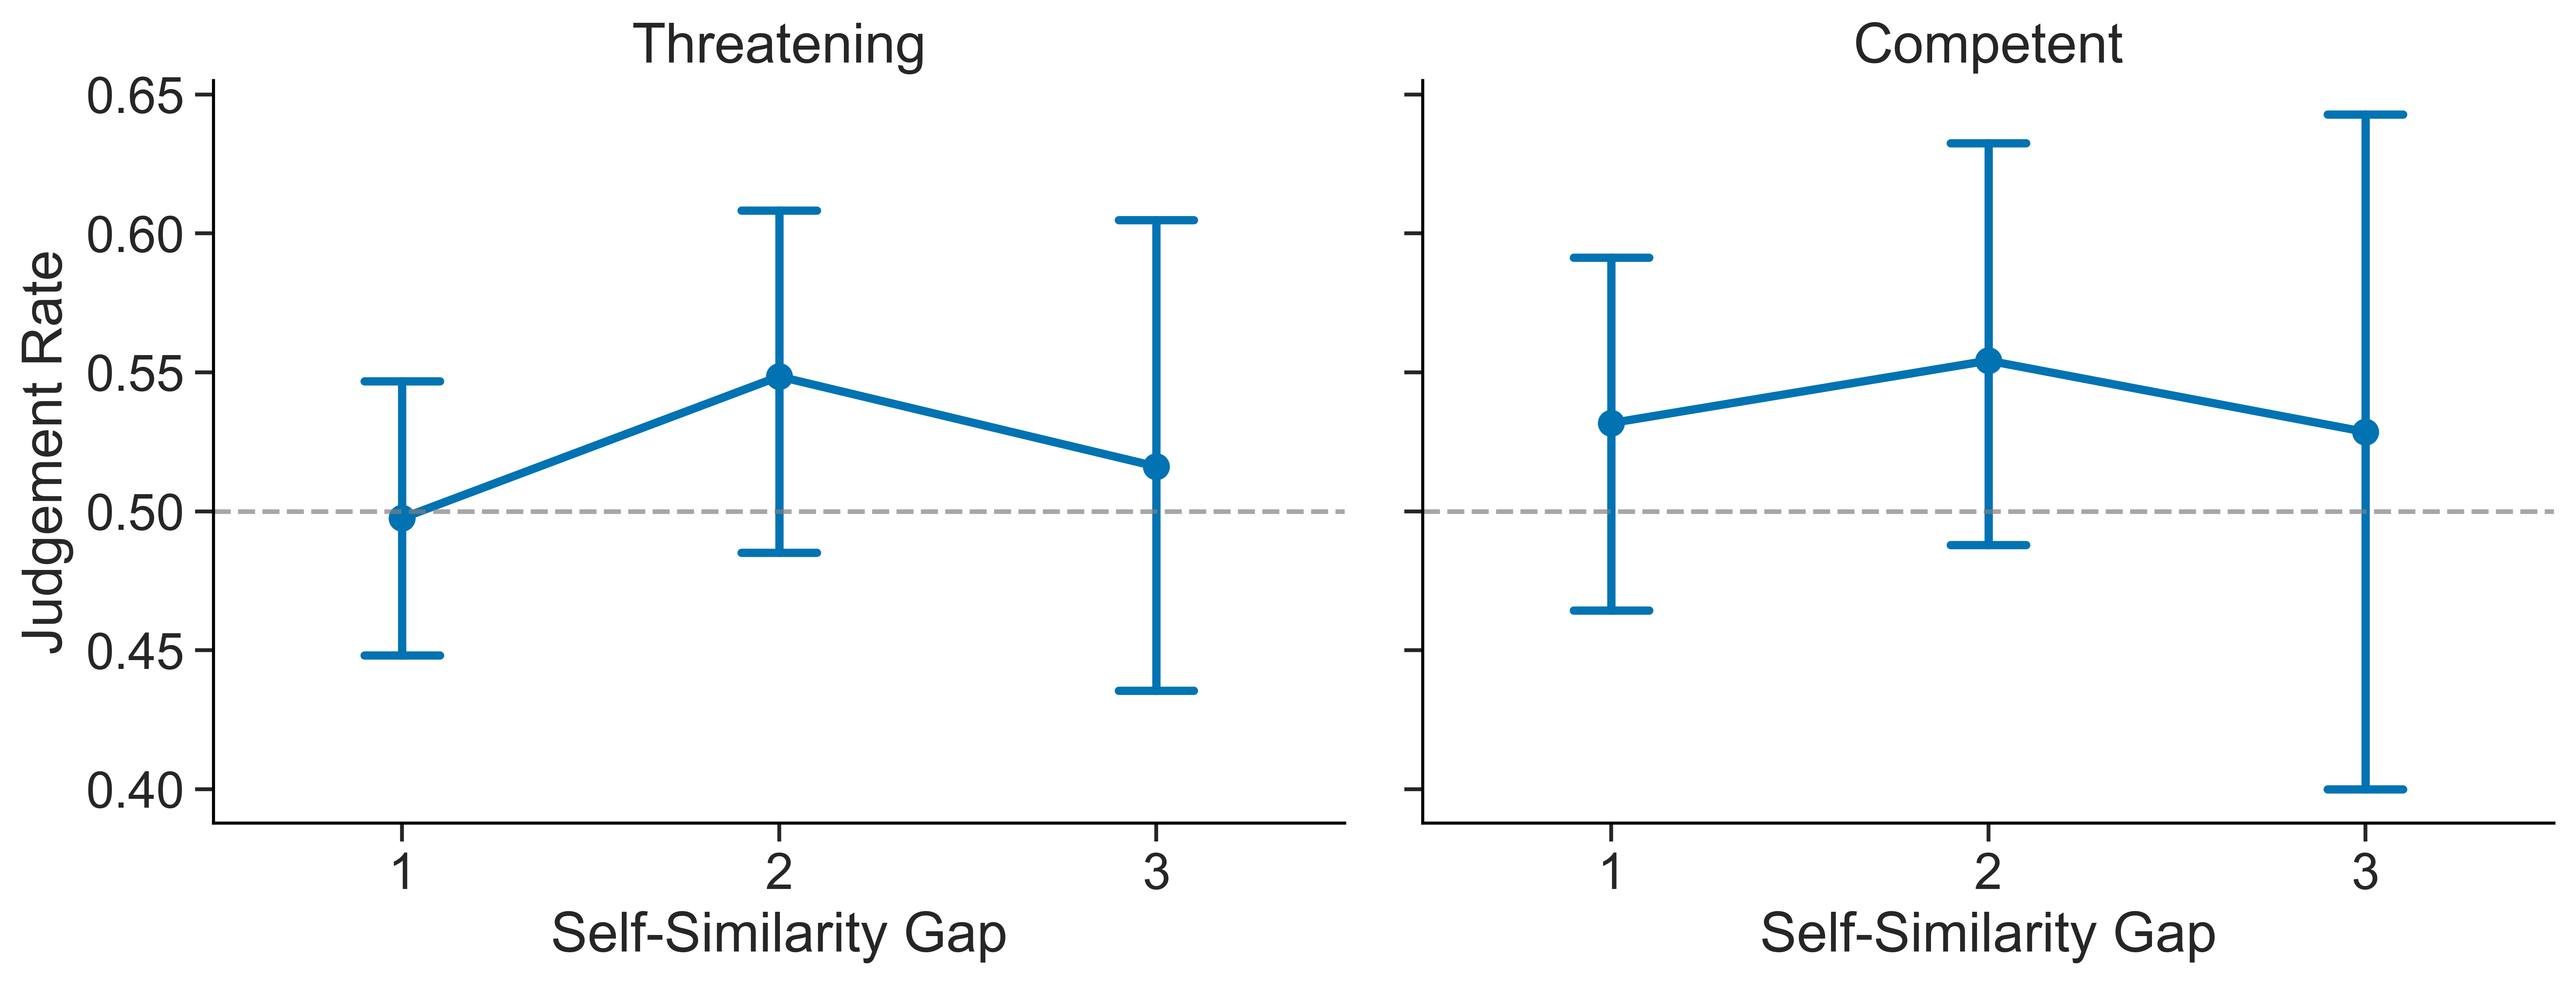
\includegraphics{attribute_figures/pointplot_chosen_vs_simDiff_condition.png}

}

\end{figure}%

Figure 6 summarizes the relationship between self-similarity gap and
participants' judgments of threat and competence. Across both judgment
types, the probability of selecting the more self-similar character
remained close to chance (50\%) at all self-similarity gaps. For threat
judgments, there was a slight increase from gap 1 to gap 2, followed by
a decrease at gap 3, but this pattern was small and inconsistent.
Confidence intervals overlapped at all levels. A similar pattern is seen
with competence judgments, where the selection rate of the more
self-similar character showed very modest variation across
self-similarity gaps and remained statistically indistinguishable from
chance. Overall, these results indicate that self-similarity does not
reliably predict judgments of either threat or competence.

\subsection{Discussion}\label{discussion-1}

These results provide little evidence that self-similarity
systematically predicts judgments of competence or threat when these
attributes are evaluated in isolation. These results should be
interpreted in light of a key difference between Experiments 1 and 2. In
Experiment 1, participants selected teammates under a framed goal
context; in Experiment 2, they made abstract, decontextualized judgments
about individual traits without any reference to team formation or task
performance. The null effects in Experiment 2 therefore rule out a
simple account in which self-similarity directly biases perceived threat
or competence across contexts. They do not show that self-similarity
could never affect evaluations when those evaluations are embedded in
the teammate-selection context itself. The present design does not
directly test that contextualized possibility. A follow-up study that
embeds threat or competence judgments within a team-based frame, or that
crosses goal type with stakes directly, would be needed to go further.

\section{General Discussion}\label{general-discussion}

This study examines how self-similarity influences team formation
decisions and demonstrates that homophily is not a fixed preference.
Across two experiments, we find that individuals preferentially select
more similar others when decisions are framed in low-stakes, affiliative
terms but that this tendency is attenuated under competitive,
performance-oriented framing. This pattern is also reflected in decision
speed, with larger self-similarity gaps associated with faster choices
in low-stakes contexts. Together, these results suggest that homophily
is sensitive to the goals of the decision context rather than operating
as a stable, unconditional bias.

The follow-up analyses narrow the interpretation of this framing effect
without identifying its mechanism directly. The trait-norm results show
that only threat avoidance was stronger under affiliative framing,
arguing against a generic account in which high stakes simply dampen all
trait-level preferences. Experiment 2 shows that self-similarity did not
predict threat or competence judgments in a neutral context, ruling out
a simple account in which self-similarity influences teammate selection
by directly biasing these impressions. And because baseline demographic
preferences remained largely stable across frames, the performance
condition does not appear to shift selection criteria wholesale.
Together, these findings are consistent with a rewards-of-interaction
account in which affiliative goals may make self-similarity a more
relevant cue for relational rewards, but they do not resolve the bundled
manipulation of stakes and goal type. A design crossing those factors
directly, or embedding trait judgments within the teammate-selection
context, would be needed to go further.

More broadly, these findings have implications for how teams are formed
in organizational and educational settings. Implicit preferences for
self-similar others may emerge in low-stakes or socially oriented
decision contexts and unintentionally shape group composition. At the
same time, the attenuation of homophily under performance-oriented task
framing suggests that such preferences are malleable and responsive to
how decisions are structured. It is also important to note that teammate
selection in this paradigm was shaped not only by self-similarity but
also by other factors, including baseline demographic preferences and
trait-based evaluations. These results also underscore that homophily
represents only one of several factors shaping team selection. When
self-similarity is downweighted, other preferences, such as baseline
demographic tendencies or trait-based evaluations, may play a larger
role in guiding decisions. Understanding how these influences interact
will be important for developing a more complete account of how team
composition emerges across different decision contexts, even as the
present paradigm isolates the specific contribution of self-similarity.

Several limitations should be noted, however. The present study employs
a unidirectional selection paradigm, in which participants choose
teammates but are not themselves subject to selection. Real-world team
formation is often reciprocal, involving negotiation and mutual
preferences. Incorporating such dynamics would allow for the examination
of how individual preferences for self-similar others translate into
actual group composition. While the present design captures individual
selection tendencies, it does not determine whether these preferences
would result in groups composed of similar others under reciprocal
choice. Another important direction is to examine how these
individual-level preferences aggregate to shape overall team
composition. While homophily is attenuated in high-stakes settings, it
remains unclear whether this reduction leads to more diverse teams or
simply reflects weaker reliance on a single heuristic. Understanding how
decision-level tendencies translate into group-level structure may help
clarify whether reduced homophily reflects a shift toward strategic
diversity-oriented selection or just a more general weakening of
self-similarity-based preferences.

Despite these limitations, the present study provides a tractable and
highly efficient framework for studying homophily in controlled
settings. A key strength of this design is its ability to isolate the
influence of self-similarity from the structure of available options,
allowing preference to be examined independently of opportunity. By
holding constant the set of alternatives and their distribution across
trials, the paradigm enables precise estimation of how contextual
factors shape selection behavior. Moreover, the use of rapid, repeated
pairwise decisions enables the recovery of individual-level sensitivity
to self-similarity with minimal data collection, and the online
implementation makes this approach both scalable and cost-effective.
Together, these features make the paradigm well-suited for
systematically investigating how contextual factors shape homophily.

\section{References}\label{references}

\phantomsection\label{refs}
\begin{CSLReferences}{1}{0}
\bibitem[\citeproctext]{ref-ajzen1974effects}
Ajzen, I. (1974). Effects of information on interpersonal attraction:
Similarity versus affective value. \emph{Journal of Personality and
Social Psychology}, \emph{29}(3), 374.

\bibitem[\citeproctext]{ref-alhazmi2017empirical}
Alhazmi, E., Horawalavithana, S., Skvoretz, J., Blackburn, J., \&
Iamnitchi, A. (2017). An empirical study on team formation in online
games. \emph{Proceedings of the 2017 IEEE/ACM International Conference
on Advances in Social Networks Analysis and Mining 2017}, 431--438.

\bibitem[\citeproctext]{ref-berscheid1969interpersonal}
Berscheid, E., \& Hatfield, E. (1969). \emph{Interpersonal attraction}
(Vol. 69). Addison-Wesley Reading, MA.

\bibitem[\citeproctext]{ref-byrne1971ubiquitous}
Byrne, D., Gouaux, C., Griffitt, W., Lamberth, J., Murakawa, N., Prasad,
M., Prasad, A., \& Ramirez III, M. (1971). The ubiquitous relationship:
Attitude similarity and attraction: A cross-cultural study. \emph{Human
Relations}, \emph{24}(3), 201--207.

\bibitem[\citeproctext]{ref-currarini2010identifying}
Currarini, S., Jackson, M. O., \& Pin, P. (2010). Identifying the roles
of race-based choice and chance in high school friendship network
formation. \emph{Proceedings of the National Academy of Sciences},
\emph{107}(11), 4857--4861.

\bibitem[\citeproctext]{ref-debruine2002facial}
DeBruine, L. M. (2002). Facial resemblance enhances trust.
\emph{Proceedings of the Royal Society of London. Series B: Biological
Sciences}, \emph{269}(1498), 1307--1312.

\bibitem[\citeproctext]{ref-debruine2004facial}
DeBruine, L. M. (2004). Facial resemblance increases the attractiveness
of same--sex faces more than other--sex faces. \emph{Proceedings of the
Royal Society of London. Series B: Biological Sciences},
\emph{271}(1552), 2085--2090.

\bibitem[\citeproctext]{ref-dehghani2016purity}
Dehghani, M., Johnson, K., Hoover, J., Sagi, E., Garten, J., Parmar, N.
J., Vaisey, S., Iliev, R., \& Graham, J. (2016). Purity homophily in
social networks. \emph{Journal of Experimental Psychology: General},
\emph{145}(3), 366.

\bibitem[\citeproctext]{ref-ertug2022does}
Ertug, G., Brennecke, J., Kovács, B., \& Zou, T. (2022). What does
homophily do? A review of the consequences of homophily. \emph{Academy
of Management Annals}, \emph{16}(1), 38--69.

\bibitem[\citeproctext]{ref-fiske2007universal}
Fiske, S. T., Cuddy, A. J., \& Glick, P. (2007). Universal dimensions of
social cognition: Warmth and competence. \emph{Trends in Cognitive
Sciences}, \emph{11}(2), 77--83.

\bibitem[\citeproctext]{ref-heine2002interjudge}
Heine, S. J., \& Renshaw, K. (2002). Interjudge agreement,
self-enhancement, and liking: Cross-cultural divergences.
\emph{Personality and Social Psychology Bulletin}, \emph{28}(5),
578--587.

\bibitem[\citeproctext]{ref-hinds2000choosing}
Hinds, P. J., Carley, K. M., Krackhardt, D., \& Wholey, D. (2000).
Choosing work group members: Balancing similarity, competence, and
familiarity. \emph{Organizational Behavior and Human Decision
Processes}, \emph{81}(2), 226--251.

\bibitem[\citeproctext]{ref-kaplan1973information}
Kaplan, M. F., \& Anderson, N. H. (1973). Information integration theory
and reinforcement theory as approaches to interpersonal attraction.
\emph{Journal of Personality and Social Psychology}, \emph{28}(3), 301.

\bibitem[\citeproctext]{ref-kossinets2009origins}
Kossinets, G., \& Watts, D. J. (2009). Origins of homophily in an
evolving social network. \emph{American Journal of Sociology},
\emph{115}(2), 405--450.

\bibitem[\citeproctext]{ref-launay2015playing}
Launay, J., \& Dunbar, R. I. (2015). Playing with strangers: Which
shared traits attract us most to new people? \emph{PloS One},
\emph{10}(6), e0129688.

\bibitem[\citeproctext]{ref-lincoln1979work}
Lincoln, J. R., \& Miller, J. (1979). Work and friendship ties in
organizations: A comparative analysis of relation networks.
\emph{Administrative Science Quarterly}, 181--199.

\bibitem[\citeproctext]{ref-ma2015chicago}
Ma, D. S., Correll, J., \& Wittenbrink, B. (2015). The chicago face
database: A free stimulus set of faces and norming data. \emph{Behavior
Research Methods}, \emph{47}, 1122--1135.

\bibitem[\citeproctext]{ref-mcmillan2022strong}
McMillan, C. (2022a). Strong and weak tie homophily in adolescent
friendship networks: An analysis of same-race and same-gender ties.
\emph{Network Science}, \emph{10}(3), 283--300.

\bibitem[\citeproctext]{ref-mcmillan2022worth}
McMillan, C. (2022b). Worth the weight: Conceptualizing and measuring
strong versus weak tie homophily. \emph{Social Networks}, \emph{68},
139--147.

\bibitem[\citeproctext]{ref-mcpherson2001birds}
McPherson, M., Smith-Lovin, L., \& Cook, J. M. (2001). Birds of a
feather: Homophily in social networks. \emph{Annual Review of
Sociology}, \emph{27}(1), 415--444.

\bibitem[\citeproctext]{ref-montoya2013meta}
Montoya, R. M., \& Horton, R. S. (2013). A meta-analytic investigation
of the processes underlying the similarity-attraction effect.
\emph{Journal of Social and Personal Relationships}, \emph{30}(1),
64--94.

\bibitem[\citeproctext]{ref-montoya2008actual}
Montoya, R. M., Horton, R. S., \& Kirchner, J. (2008). Is actual
similarity necessary for attraction? A meta-analysis of actual and
perceived similarity. \emph{Journal of Social and Personal
Relationships}, \emph{25}(6), 889--922.

\bibitem[\citeproctext]{ref-nakano2022you}
Nakano, T., \& Yamamoto, T. (2022). You trust a face like yours.
\emph{Humanities and Social Sciences Communications}, \emph{9}(1), 1--6.

\bibitem[\citeproctext]{ref-novak1968rejection}
Novak, D. W., \& Lerner, M. J. (1968). Rejection as a consequence of
perceived similarity. \emph{Journal of Personality and Social
Psychology}, \emph{9}(2p1), 147.

\bibitem[\citeproctext]{ref-olivola2010elected}
Olivola, C. Y., \& Todorov, A. (2010). Elected in 100 milliseconds:
Appearance-based trait inferences and voting. \emph{Journal of Nonverbal
Behavior}, \emph{34}, 83--110.

\bibitem[\citeproctext]{ref-oosterhof2008functional}
Oosterhof, N. N., \& Todorov, A. (2008). The functional basis of face
evaluation. \emph{Proceedings of the National Academy of Sciences},
\emph{105}(32), 11087--11092.

\bibitem[\citeproctext]{ref-reagans2001networks}
Reagans, R., \& Zuckerman, E. W. (2001). Networks, diversity, and
productivity: The social capital of corporate r\&d teams.
\emph{Organization Science}, \emph{12}(4), 502--517.

\bibitem[\citeproctext]{ref-rivera2012hiring}
Rivera, L. A. (2012). Hiring as cultural matching: The case of elite
professional service firms. \emph{American Sociological Review},
\emph{77}(6), 999--1022.

\bibitem[\citeproctext]{ref-ruef2003structure}
Ruef, M., Aldrich, H. E., \& Carter, N. M. (2003). The structure of
founding teams: Homophily, strong ties, and isolation among US
entrepreneurs. \emph{American Sociological Review}, \emph{68}(2),
195--222.

\bibitem[\citeproctext]{ref-stallen2023partner}
Stallen, M., Snijder, L. L., Gross, J., Hilbert, L. P., \& De Dreu, C.
K. (2023). Partner choice and cooperation in social dilemmas can
increase resource inequality. \emph{Nature Communications},
\emph{14}(1), 6432.

\bibitem[\citeproctext]{ref-tajfel1979integrative}
Tajfel, H., Turner, J. C., Austin, W. G., \& Worchel, S. (1979). An
integrative theory of intergroup conflict. \emph{Organizational
Identity: A Reader}, \emph{56}(65), 9780203505984--9780203505916.

\bibitem[\citeproctext]{ref-willis2006first}
Willis, J., \& Todorov, A. (2006). First impressions: Making up your
mind after a 100-ms exposure to a face. \emph{Psychological Science},
\emph{17}(7), 592--598.

\bibitem[\citeproctext]{ref-wimmer2010beyond}
Wimmer, A., \& Lewis, K. (2010). Beyond and below racial homophily: ERG
models of a friendship network documented on facebook. \emph{American
Journal of Sociology}, \emph{116}(2), 583--642.

\bibitem[\citeproctext]{ref-yamagishi1999bounded}
Yamagishi, T. (1999). Bounded generalized reciprocity: Ingroup boasting
and ingroup favoritism. \emph{Advances in Group Processes}, \emph{16},
161.

\bibitem[\citeproctext]{ref-zebrowitz2017first}
Zebrowitz, L. A. (2017). First impressions from faces. \emph{Current
Directions in Psychological Science}, \emph{26}(3), 237--242.

\bibitem[\citeproctext]{ref-zell2020better}
Zell, E., Strickhouser, J. E., Sedikides, C., \& Alicke, M. D. (2020).
The better-than-average effect in comparative self-evaluation: A
comprehensive review and meta-analysis. \emph{Psychological Bulletin},
\emph{146}(2), 118.

\end{CSLReferences}

\subsection{Supplementary Materials}\label{supplementary-materials}

\subsubsection{Tables}\label{tables}

\begin{table}

{\caption{{Probability of selecting the more-similar player by
similarity difference and Condition.}{\label{tbl-condition}}}
\vspace{-20pt}}

\begin{longtable}[]{@{}
  >{\centering\arraybackslash}p{(\columnwidth - 8\tabcolsep) * \real{0.2632}}
  >{\centering\arraybackslash}p{(\columnwidth - 8\tabcolsep) * \real{0.2316}}
  >{\raggedleft\arraybackslash}p{(\columnwidth - 8\tabcolsep) * \real{0.1684}}
  >{\raggedleft\arraybackslash}p{(\columnwidth - 8\tabcolsep) * \real{0.1684}}
  >{\raggedleft\arraybackslash}p{(\columnwidth - 8\tabcolsep) * \real{0.1684}}@{}}
\toprule\noalign{}
\begin{minipage}[b]{\linewidth}\centering
Self-Similarity Gap
\end{minipage} & \begin{minipage}[b]{\linewidth}\centering
Condition
\end{minipage} & \begin{minipage}[b]{\linewidth}\raggedleft
Preference Rate
\end{minipage} & \begin{minipage}[b]{\linewidth}\raggedleft
95\% CI (Lower)
\end{minipage} & \begin{minipage}[b]{\linewidth}\raggedleft
95\% CI (Upper)
\end{minipage} \\
\midrule\noalign{}
\endhead
\bottomrule\noalign{}
\endlastfoot
1 & High-Stakes / Performance Frame & 0.524 & 0.485 & 0.564 \\
1 & Low-Stakes / Affiliative Frame & 0.586 & 0.545 & 0.627 \\
2 & High-Stakes / Performance Frame & 0.546 & 0.500 & 0.595 \\
2 & Low-Stakes / Affiliative Frame & 0.657 & 0.608 & 0.706 \\
3 & High-Stakes / Performance Frame & 0.623 & 0.550 & 0.691 \\
3 & Low-Stakes / Affiliative Frame & 0.708 & 0.643 & 0.774 \\
\end{longtable}

\end{table}

\begin{table}

{\caption{{Fixed effects from the participant-slope decomposed follow-up
model replacing the summed self-similarity gap with separate race-,
age-, and gender-match differences. Positive coefficients indicate that
the focal candidate was more likely to be chosen when they were
relatively more similar to the participant than the alternative on that
dimension.}{\label{tbl-multisimdiff-components}}}
\vspace{-20pt}}

\begin{longtable}[]{@{}
  >{\raggedright\arraybackslash}p{(\columnwidth - 8\tabcolsep) * \real{0.2000}}
  >{\raggedleft\arraybackslash}p{(\columnwidth - 8\tabcolsep) * \real{0.2000}}
  >{\raggedleft\arraybackslash}p{(\columnwidth - 8\tabcolsep) * \real{0.2000}}
  >{\raggedleft\arraybackslash}p{(\columnwidth - 8\tabcolsep) * \real{0.2000}}
  >{\raggedright\arraybackslash}p{(\columnwidth - 8\tabcolsep) * \real{0.2000}}@{}}
\toprule\noalign{}
\begin{minipage}[b]{\linewidth}\raggedright
Fixed Effect
\end{minipage} & \begin{minipage}[b]{\linewidth}\raggedleft
Estimate (beta)
\end{minipage} & \begin{minipage}[b]{\linewidth}\raggedleft
SE
\end{minipage} & \begin{minipage}[b]{\linewidth}\raggedleft
z
\end{minipage} & \begin{minipage}[b]{\linewidth}\raggedright
p
\end{minipage} \\
\midrule\noalign{}
\endhead
\bottomrule\noalign{}
\endlastfoot
(Intercept) & 0.021 & 0.067 & 0.314 & 0.754 \\
Race-match difference & 0.885 & 0.259 & 3.414 & \textbf{\textless{}
.001} \\
Age-match difference & 0.602 & 0.264 & 2.277 & \textbf{0.023} \\
Gender-match difference & 0.459 & 0.293 & 1.567 & 0.117 \\
High-Stakes / Performance frame & -0.025 & 0.079 & -0.312 & 0.755 \\
Race-match difference × High-Stakes / Performance frame & -0.548 & 0.354
& -1.548 & 0.122 \\
Age-match difference × High-Stakes / Performance frame & -0.475 & 0.362
& -1.312 & 0.190 \\
Gender-match difference × High-Stakes / Performance frame & -0.168 &
0.403 & -0.418 & 0.676 \\
\end{longtable}

\end{table}

\begin{table}

{\caption{{Simple effects from the participant-race follow-up to the
demographic-only model. Each row reports the candidate-race contrast
relative to Black faces within one participant-race group, based on a
logistic mixed model that also controlled for target age, target gender,
framing condition, and a random intercept for character. Positive
coefficients indicate that the focal candidate was more likely to be
chosen than a Black face within that participant group; negative
coefficients indicate relative avoidance. Multiracial and Other
participants were excluded from this follow-up because each group
contained a single participant.}{\label{tbl-demo-participant-race}}}
\vspace{-20pt}}

\begin{longtable}[]{@{}
  >{\raggedright\arraybackslash}p{(\columnwidth - 10\tabcolsep) * \real{0.1667}}
  >{\raggedright\arraybackslash}p{(\columnwidth - 10\tabcolsep) * \real{0.1667}}
  >{\raggedleft\arraybackslash}p{(\columnwidth - 10\tabcolsep) * \real{0.1667}}
  >{\raggedleft\arraybackslash}p{(\columnwidth - 10\tabcolsep) * \real{0.1667}}
  >{\raggedleft\arraybackslash}p{(\columnwidth - 10\tabcolsep) * \real{0.1667}}
  >{\raggedright\arraybackslash}p{(\columnwidth - 10\tabcolsep) * \real{0.1667}}@{}}
\toprule\noalign{}
\begin{minipage}[b]{\linewidth}\raggedright
Participant Race
\end{minipage} & \begin{minipage}[b]{\linewidth}\raggedright
Candidate Race Contrast
\end{minipage} & \begin{minipage}[b]{\linewidth}\raggedleft
Estimate (beta)
\end{minipage} & \begin{minipage}[b]{\linewidth}\raggedleft
SE
\end{minipage} & \begin{minipage}[b]{\linewidth}\raggedleft
z
\end{minipage} & \begin{minipage}[b]{\linewidth}\raggedright
p
\end{minipage} \\
\midrule\noalign{}
\endhead
\bottomrule\noalign{}
\endlastfoot
Black & East-Asian vs.~Black & -0.261 & 0.296 & -0.881 & 0.378 \\
Black & Latino vs.~Black & -0.640 & 0.304 & -2.103 & \textbf{0.035} \\
Black & South-Asian vs.~Black & -1.273 & 0.304 & -4.190 &
\textbf{\textless{} .001} \\
Black & White vs.~Black & -1.644 & 0.295 & -5.581 & \textbf{\textless{}
.001} \\
East/Southeast Asian & East-Asian vs.~Black & 0.805 & 0.250 & 3.216 &
\textbf{0.001} \\
East/Southeast Asian & Latino vs.~Black & -0.272 & 0.303 & -0.896 &
0.370 \\
East/Southeast Asian & South-Asian vs.~Black & 0.383 & 0.289 & 1.325 &
0.185 \\
East/Southeast Asian & White vs.~Black & -0.058 & 0.310 & -0.187 &
0.851 \\
Hispanic/Latine/Latinx & East-Asian vs.~Black & -0.175 & 0.376 & -0.465
& 0.642 \\
Hispanic/Latine/Latinx & Latino vs.~Black & 0.131 & 0.329 & 0.399 &
0.690 \\
Hispanic/Latine/Latinx & South-Asian vs.~Black & -0.598 & 0.393 & -1.521
& 0.128 \\
Hispanic/Latine/Latinx & White vs.~Black & -0.488 & 0.361 & -1.350 &
0.177 \\
South Asian & East-Asian vs.~Black & 0.449 & 0.440 & 1.018 & 0.308 \\
South Asian & Latino vs.~Black & -0.332 & 0.470 & -0.706 & 0.480 \\
South Asian & South-Asian vs.~Black & -0.185 & 0.423 & -0.438 & 0.661 \\
South Asian & White vs.~Black & -1.033 & 0.456 & -2.266 &
\textbf{0.023} \\
White & East-Asian vs.~Black & 0.165 & 0.274 & 0.602 & 0.548 \\
White & Latino vs.~Black & -0.211 & 0.290 & -0.726 & 0.468 \\
White & South-Asian vs.~Black & -0.374 & 0.281 & -1.332 & 0.183 \\
White & White vs.~Black & -0.124 & 0.235 & -0.529 & 0.597 \\
\end{longtable}

\end{table}

\begin{table}

{\caption{{Fixed effects from six separate trait-norm logistic mixed
models. Each model regressed whether the focal face was chosen on the
signed focal-minus-opponent difference score for one CFD trait, framing
condition, and their interaction, with a random intercept for character.
Positive baseline coefficients indicate that higher values of the focal
trait increased selection in the affiliative frame; positive interaction
coefficients indicate attenuation or reversal of that effect in the
high-stakes/performance frame. \texttt{p\_adj} reports
Benjamini-Hochberg adjusted p-values across the six trait-by-frame
interaction tests.}{\label{tbl-trait-norms}}}
\vspace{-20pt}}

\begin{longtable}[]{@{}
  >{\raggedright\arraybackslash}p{(\columnwidth - 20\tabcolsep) * \real{0.0909}}
  >{\raggedleft\arraybackslash}p{(\columnwidth - 20\tabcolsep) * \real{0.0909}}
  >{\raggedleft\arraybackslash}p{(\columnwidth - 20\tabcolsep) * \real{0.0909}}
  >{\raggedleft\arraybackslash}p{(\columnwidth - 20\tabcolsep) * \real{0.0909}}
  >{\raggedleft\arraybackslash}p{(\columnwidth - 20\tabcolsep) * \real{0.0909}}
  >{\raggedright\arraybackslash}p{(\columnwidth - 20\tabcolsep) * \real{0.0909}}
  >{\raggedleft\arraybackslash}p{(\columnwidth - 20\tabcolsep) * \real{0.0909}}
  >{\raggedleft\arraybackslash}p{(\columnwidth - 20\tabcolsep) * \real{0.0909}}
  >{\raggedleft\arraybackslash}p{(\columnwidth - 20\tabcolsep) * \real{0.0909}}
  >{\raggedright\arraybackslash}p{(\columnwidth - 20\tabcolsep) * \real{0.0909}}
  >{\raggedright\arraybackslash}p{(\columnwidth - 20\tabcolsep) * \real{0.0909}}@{}}
\toprule\noalign{}
\begin{minipage}[b]{\linewidth}\raggedright
Trait
\end{minipage} & \begin{minipage}[b]{\linewidth}\raggedleft
N
\end{minipage} & \begin{minipage}[b]{\linewidth}\raggedleft
Trait Difference (beta)
\end{minipage} & \begin{minipage}[b]{\linewidth}\raggedleft
SE
\end{minipage} & \begin{minipage}[b]{\linewidth}\raggedleft
z
\end{minipage} & \begin{minipage}[b]{\linewidth}\raggedright
p
\end{minipage} & \begin{minipage}[b]{\linewidth}\raggedleft
Trait Difference × High-Stakes (beta)
\end{minipage} & \begin{minipage}[b]{\linewidth}\raggedleft
SE
\end{minipage} & \begin{minipage}[b]{\linewidth}\raggedleft
z
\end{minipage} & \begin{minipage}[b]{\linewidth}\raggedright
p
\end{minipage} & \begin{minipage}[b]{\linewidth}\raggedright
p\_adj
\end{minipage} \\
\midrule\noalign{}
\endhead
\bottomrule\noalign{}
\endlastfoot
Attractiveness & 5544 & 0.406 & 0.048 & 8.501 & \textbf{\textless{}
.001} & -0.130 & 0.060 & -2.178 & \textbf{0.029} & 0.059 \\
Dominance & 3802 & -0.068 & 0.063 & -1.081 & 0.280 & -0.099 & 0.080 &
-1.231 & 0.218 & 0.218 \\
Happiness & 5544 & 0.289 & 0.050 & 5.747 & \textbf{\textless{} .001} &
-0.084 & 0.063 & -1.341 & 0.180 & 0.216 \\
Sadness & 5544 & -0.338 & 0.050 & -6.699 & \textbf{\textless{} .001} &
0.174 & 0.064 & 2.721 & \textbf{0.007} & 0.029 \\
Threat & 5544 & -0.435 & 0.054 & -8.002 & \textbf{\textless{} .001} &
0.184 & 0.071 & 2.591 & \textbf{0.010} & 0.029 \\
Trustworthiness & 5544 & 0.379 & 0.067 & 5.675 & \textbf{\textless{}
.001} & -0.115 & 0.083 & -1.381 & 0.167 & 0.216 \\
\end{longtable}

\end{table}

\begin{table}

{\caption{{Probability of preferring the focal player by similarity of
focal and other player to participant.}{\label{tbl-heatmap}}}
\vspace{-20pt}}

\begin{longtable}[]{@{}ccccc@{}}
\toprule\noalign{}
Other ~Focal & 0 & 1 & 2 & 3 \\
\midrule\noalign{}
\endhead
\bottomrule\noalign{}
\endlastfoot
0 & 0.500 & 0.535 & 0.582 & 0.663 \\
1 & & 0.500 & 0.520 & 0.617 \\
2 & & & 0.500 & 0.616 \\
3 & & & & 0.500 \\
\end{longtable}

\end{table}

\begin{table}

{\caption{{Mean reaction time (milliseconds) as a function of
self-similarity gap.}{\label{tbl-rt-simdiff}}}
\vspace{-20pt}}

\begin{longtable}[]{@{}
  >{\centering\arraybackslash}p{(\columnwidth - 6\tabcolsep) * \real{0.3182}}
  >{\centering\arraybackslash}p{(\columnwidth - 6\tabcolsep) * \real{0.1970}}
  >{\raggedleft\arraybackslash}p{(\columnwidth - 6\tabcolsep) * \real{0.2424}}
  >{\raggedleft\arraybackslash}p{(\columnwidth - 6\tabcolsep) * \real{0.2424}}@{}}
\toprule\noalign{}
\begin{minipage}[b]{\linewidth}\centering
Self-Similarity Gap
\end{minipage} & \begin{minipage}[b]{\linewidth}\centering
Mean RT (ms)
\end{minipage} & \begin{minipage}[b]{\linewidth}\raggedleft
95 \% CI (Lower)
\end{minipage} & \begin{minipage}[b]{\linewidth}\raggedleft
95 \% CI (Upper)
\end{minipage} \\
\midrule\noalign{}
\endhead
\bottomrule\noalign{}
\endlastfoot
1 & 2599.290 & 2505.245 & 2699.081 \\
2 & 2487.619 & 2380.222 & 2594.126 \\
3 & 2328.423 & 2168.046 & 2500.506 \\
\end{longtable}

\end{table}

\begin{table}

{\caption{{Mean reaction time (milliseconds) by self-similarity gap and
Condition.}{\label{tbl-rt-simDiff-cond}}}
\vspace{-20pt}}

\begin{longtable}[]{@{}
  >{\centering\arraybackslash}p{(\columnwidth - 8\tabcolsep) * \real{0.2564}}
  >{\centering\arraybackslash}p{(\columnwidth - 8\tabcolsep) * \real{0.1538}}
  >{\raggedleft\arraybackslash}p{(\columnwidth - 8\tabcolsep) * \real{0.1795}}
  >{\raggedleft\arraybackslash}p{(\columnwidth - 8\tabcolsep) * \real{0.2051}}
  >{\raggedleft\arraybackslash}p{(\columnwidth - 8\tabcolsep) * \real{0.2051}}@{}}
\toprule\noalign{}
\begin{minipage}[b]{\linewidth}\centering
Self-Similarity Gap
\end{minipage} & \begin{minipage}[b]{\linewidth}\centering
Condition
\end{minipage} & \begin{minipage}[b]{\linewidth}\raggedleft
Mean RT (ms)
\end{minipage} & \begin{minipage}[b]{\linewidth}\raggedleft
95 \% CI (Lower)
\end{minipage} & \begin{minipage}[b]{\linewidth}\raggedleft
95 \% CI (Upper)
\end{minipage} \\
\midrule\noalign{}
\endhead
\bottomrule\noalign{}
\endlastfoot
1 & High-Stakes / Performance Frame & 2517.5 & 2387.5 & 2656.9 \\
1 & Low-Stakes / Affiliative Frame & 2690.6 & 2561.2 & 2825.6 \\
2 & High-Stakes / Performance Frame & 2397.9 & 2246.3 & 2552.6 \\
2 & Low-Stakes / Affiliative Frame & 2588.4 & 2428.6 & 2749.0 \\
3 & High-Stakes / Performance Frame & 2309.6 & 2073.2 & 2569.5 \\
3 & Low-Stakes / Affiliative Frame & 2349.2 & 2120.5 & 2593.6 \\
\end{longtable}

\end{table}

\subsubsection{Instructions}\label{instructions}

\paragraph{General Instructions.}\label{general-instructions}

\begin{quote}
Hello! Thank you for participating in this study. Your participation is
for research and is entirely voluntary. The study should take under 10
minutes to complete. The general purpose of this study is to better
understand social grouping behavior. The complete purpose of the study
will be explained after it is concluded. Contact information will be
provided at the end for any further questions or clarifications. If you
would like to participate in this study, please confirm that you are
eighteen years of age or older.
\end{quote}

\begin{quote}
Thank you for participating in this research study. Please enter your
information on the next page and read the instructions that follow. Some
details about this study may not be known until the study is completed.
\end{quote}

\begin{quote}
Team Selection - Pairwise Preferences For privacy reasons, each
participant in the player lobby, including yourself, has been assigned a
unique, generated icon based on their demographics. On the following
screens, you will see pairs of players in the queue; please choose the
player you would prefer to have on your team from each pair. Thank you
for your participation! Your data will help us better understand social
grouping behavior in competitive and non-competitive environments.
\end{quote}

\paragraph{Instructions Specific to Casual Condition of Experiment
1.}\label{instructions-specific-to-casual-condition-of-experiment-1}

\begin{quote}
You are about to participate in a team activity focused on improving a
local community space. Your team will develop ideas and plans to enhance
the local park, aiming to make it a better place for everyone. This is
an opportunity to collaborate, share ideas, and contribute positively to
your community in a relaxed setting.
\end{quote}

\begin{quote}
You have been randomly selected as the team leader. Before the game
begins, you will have the opportunity to select your preferences for
team members. Select those whom you believe will make the collaboration
enjoyable and productive. Based on your preferences in the drafts, we
will create teams such that your most preferred players will form your
team, and your least preferred players will form another team working on
similar plans.
\end{quote}

\begin{quote}
You are selecting a team for a team activity focused on improving a
local community space. Your team will develop ideas and plans to enhance
the local park, aiming to make it a better place for everyone. This is
an opportunity to collaborate, share ideas, and contribute positively to
your community in a relaxed setting.
\end{quote}

\paragraph{Instructions Specific to Competitive Condition of Experiment
1.}\label{instructions-specific-to-competitive-condition-of-experiment-1}

\begin{quote}
You are about to participate in a team competition focused on improving
a local community space. Your team must develop an innovative and
impactful proposal to enhance the local park, competing directly against
another team for a substantial grant from the city council. The team
with the best proposal will receive funding for implementing their
ideas.
\end{quote}

\begin{quote}
You have been randomly selected as the team leader. Before the game
begins, you will have the opportunity to select your preferences for
team members. Select those whom you believe will maximize your team's
chances of winning the grant. Based on your preferences in the drafts,
we will create teams such that your most preferred players will form
your team, and your least preferred players will form the rival team.
\end{quote}

\begin{quote}
You are selecting a team for a team competition focused on improving a
local community space. Your team must develop an innovative and
impactful proposal to enhance the local park, competing directly against
another team for a substantial grant from the city council. The team
with the best proposal will receive funding for implementing their
ideas.
\end{quote}

\paragraph{Instructions Specific to Experiment
2.}\label{instructions-specific-to-experiment-2}

Task-specific instructions were identical across conditions of
Experiment 2, with the only difference being whether participants were
asked to judge which character appeared more \textbf{Threatening} or
more \textbf{Competent}. The same pairwise selection format was used,
with characters presented side by side and participants clicking to
indicate their choice.

\begin{quote}
Threat (Competence) Perception Task In this task, you will see pairs of
characters. Your job is to choose the one you find more Threatening
(Competent). There are no right or wrong answers; we want you to reflect
and convey your honest impressions. Press ``Next'' to begin. Use the
buttons on each side to indicate your choice. Please respond as
accurately to your impressions as you can.
\end{quote}

\begin{quote}
Pairwise Judgments On each screen, you'll see two characters. Please
choose the one you judge to be more \textbf{Threatening}
(\textbf{Competent}). Each character has been assigned a unique,
generated icon based on their demographics. Click the character you
judge to be more \textbf{Threatening} (\textbf{Competent}).
\end{quote}






\end{document}
